% Chapter Electrodes

\chapter{Simulation and Experimental Studies of the detectors RED80 and REDN1} % Main chapter title

\label{ChapterElectrodesExperimental} % Change X to a consecutive number; for referencing this chapter elsewhere, use \ref{ChapterX}

%----------------------------------------------------------------------------------------
%	BEGING CHAPTER
%----------------------------------------------------------------------------------------

% Introduction

In this chapter, the electrostatics simulation are compared to the experimental data collected from the operation of the detectors RED80 and REDN1.
Their designs differ from the already presented PL38 and FID38 designs.
Consequently, the first section is dedicated to the presentation of the detectors RED80 and REDN1, their numerical simulation and their predicted performance for the ionization channel.
The section exposes the processing and analysis pipelines used to treat the experimental data and extract observable quantities which can be compared to the simulations.
The actual confrontation of the results is presented in the last and third section.


\section{Electrostatic Simulation of the detectors RED80 and REDN1}

The detectors RED80 and REDN1 were both based on cylindrical germanium crystals of height $H_{Ge} = \SI{10}{\mm}$ and radius $R_{Ge} = \SI{15}{\mm}$. Due to technological constraints, these germanium cylinders feature a round filet on their corners with an estimated radius between \SI{200}{\micro\metre} and \SI{300}{\micro\metre}. The figure \ref{fig:photo-redn1-red80} displays the photos of the detectors. In both cliches, the covers of the copper chassis are removed as to allow the completion of the cabling of the thermal sensor and the electrodes. The incomplete chassis visible on the photos are spaced by a distance $d_{Cu} = \SI{3}{\mm}$ from the surface of the crystals. The germanium absorber are maintained by six Teflon clamps.
These detectors possesses the two energy measurement channels, heat and ionization, described in paragraph \ref{par:detector-principle}. The NTD thermal sensors, used for the heat channel, are glued at the center of the top surface of the crystals. These thermistances are linked with several gold wires to conductive tracks above the crystal. These gold wires assured the electric cabling of the NTD as well as the thermalization of the germanium crystal. The ionization channel consists in electrodes made out of aluminium pads and rings deposited on the germanium surface as explained in paragraph \ref{par:aluminium-deposition}. In the case of REDN1, the aluminium rings are linked together using wire bridges. The electrodes are wired to conductive tracks on the chassis with aluminium wires as to prevent thermal leak through them.

\begin{figure}
\centering
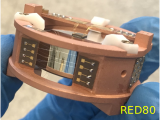
\includegraphics[align=c, scale=0.5]{Figures/ElectrodesExperimental/photo_red80_v2.pdf}
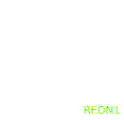
\includegraphics[align=c, scale=0.5]{Figures/ElectrodesExperimental/photo_redn1_v2.pdf}
\caption{Photos of the detector RED80 and REDN1 taken during their montage. The covers of the copper chassis are removed to finish the cabling.}
\label{fig:photo-redn1-red80}
\end{figure}

Each detector has its own particularities which are assessed in the following paragraphs \ref{par:red80-presentation} and \ref{par:redn1-presentation} dedicated to the design and the electrostatics simulation of RED80 and REDN1 respectively.


\subsection{RED80 detector}
\label{par:red80-presentation}

The description of RED80 is accompanied with the figure $\ref{fig:red80-scheme}$ displaying a cross-section scheme of the detector. This scheme is used as reference for the electrostatics simulation. The scheme is not at scale and all the dimensions used in the simulation are listed in the table \ref{tab:red80-default-parameters}.
% copper chassis
The copper chassis is modeled by an exterior electrically grounded rectangle. The germanium crystal is held separated from the germanium crystal by vacuum represented by the light blue surrounding volume.
% teflon clamps
The Teflon clamps are not represented in the scheme and are not a part of the simulation as discussed in paragraph \ref{par:simulation-limitations}.
% heat channel
The heat channel of RED80 consists of a GeNTD thermistance labeled K58. Its dimensions are the larger Edelweiss standard of \SI{4 x 4 x 0.45}{\mm}. It is glued on aluminium at the center of the top surface as represented by the white rectangle. Although represented, the NTD is not simulated as discussed in paragraph \ref{par:simulation-limitations}.
% ionization channel
The ionization channel consists in four electrodes labeled $A$ through $D$ separated in pairs of collecting and guard electrodes. Each aluminium deposit is labeled on the scheme $\ref{fig:red80-scheme}$ according to the electrode it is attributed to.
The main electrodes are $B$ and $D$. They consists of two planar full aluminium electrodes of radius $r_{center} = \SI{13.5}{\mm}$ centered on the top and bottom surfaces of the germanium crystal. The role of these electrodes is to collect the majority of the drifting charges produced in the crystal. As such, they are deemed "collect electrodes".
The auxiliary electrodes are $A$ and $C$. They are formed by two pairs of circular rings of width $w_{Al}=\SI{100}{\micro\meter}$ deposited on the lateral surface of the germanium crystal. In each pair, the rings are separated by the lateral spacing $d_{lat}=\SI{2.4}{\mm}$, from their center. The two pairs are spaced by the equatorial distance $d_{eq} = \SI{1}{\mm}$, from the center of the center-most rings. The function of these electrodes is to collect any charges in the periphery of the crystal as to tag any surface recoil similarly to veto electrodes principles presented in paragraph \ref{par:veto-electrode-principle}. These electrodes are deemed "guard electrodes" as opposed to the veto ones. The difference holds in their polarization and in the direction of the electric field being the same between the collect and the guard electrodes.
% Equator offset
One should note that the guard electrodes are not centered on the equator of the crystal, represented by the finely-dashed horizontal line passing through the origin $(0,0)$ in the scheme \ref{fig:red80-scheme}. Instead, the axis of mirror symmetry for the guard electrodes is the sparsely-dashed  horizontal line passing through the coordinates $(0, z_{eq})=(0, -0.5)\si{\mm}$. This is the result of an offset in height of the mask used during the deposition of the aluminium rings. While this feature is unintentional as it induces an slight asymmetry in the design of RED80, it shall provides interesting insights considering the intrinsic asymmetry of the electron and hole drift in the semi-conducting germanium as discussed in paragraph \ref{par:charge-drift}.

\begin{figure}
\centering
\includegraphics[scale=1]{Figures/ElectrodesExperimental/scheme_red80.pdf}
\caption{Cross-section scheme of the RED80 detector. This scheme is not at scale and the main dimensions are listed in the table \ref{tab:red80-default-parameters}. The dashed horizontal lines are axis of symmetry: finely-dashed through $(0,0)$ is for the crystal, sparsely-dashed through $(0, z_{eq})=(0, -0.5)\si{\mm}$  is for the guard rings $A,C$. The electrically grounded rectangle is the cooper chassis separated from the germanium crystal by vacuum in light blue. The aluminium pads and rings are represented in black at the surface of the crystal and labeled according to their electrode of attribution. The default potential of the electrodes are $(V_A, V_B, V_C, V_D) = (+1, +1, -1, -1) \si{\volt}$. The colored volumes inside the crystal are drawn from electric field lines with common start and end points.}
\label{fig:red80-scheme}
\end{figure}

\begin{table}[]
\centering
%\resizebox{\textwidth}{!}{%
\begin{tabular}{l c S}
Parameter                                   & Symbol        & {Default Value} \\ \hline \hline
Ge crystal Height                           & $H_{Ge}$      & \SI{10}{\mm}  \\
Ge crystal Radius                           & $R_{Ge}$      & \SI{15}{\mm}    \\
Distance between crystal and copper chassis & $d_{Cu}$      & \SI{3}{\mm}     \\
Aluminium Deposit Thickness                         & $h_{Al}$      & \SI{1}{\micro\meter}   \\
Width of the Lateral Rings                      & $w_{Al}$      & \SI{80}{\micro\meter}  \\
Radius of the Planar Electrode Pad  & $r_{center}$   & \SI{13.5}{\mm}   \\
Width of bare Ge crystal on edge     & $w_{bare}$    & \SI{1.5}{\mm}  \\
Spacing between Lateral Rings          & $d_{lat}$  & \SI{2.4}{\mm}  \\
Equatorial distance						& $d_{eq}$	& \SI{1.2}{\mm} \\
Offset on Equator Height				& $z_{eq}$	& \SI{-0.5}{\mm} \\
Main Voltage Bias                           & $V_{bias}$    & \SI{2}{\volt}      \\
Symmetric factor of the voltage bias        & $S_{bias}$    & {$0.5$}         
\end{tabular}
%}%
\caption{Parameter values for the design and default polarization of RED80.}
\label{tab:red80-default-parameters}
\end{table}

% Capacitance
The electrostatic simulation of the presented geometry yields the capacitance matrices  of the detector RED80. The convention regarding indexes introduced in the chapter \ref{ChapterElectrodes} is still in use. Each electrode is attributed to an index such that:
\begin{equation}
\label{eq:indexes-convention}
\{ A, B, C, D \} \Leftrightarrow \{ 1, 2, 3, 4 \}
\end{equation}
In this light, the Maxwell capacitance matrix associated with the electrodes of RED80 is evaluated to:
\begin{equation}
\label{eq:redn1-maxwell}
\bm{C} = 
\begin{pmatrix}
  13.93 & -6.32 & -3.89 & -2.57\\
  -6.32 & 17.17 & -1.91 & -6.06\\
  -3.89 & -1.91 & 14.25 & -7.28\\
  -2.57 & -6.06 & -7.28 & 18.61\\
\end{pmatrix}
\times \SI{e-12}{\farad}
\end{equation}
Using the equations \ref{eq:maxwell-to-mutual}, the mutual capacitance matrix of RED80 is evaluated to:
\begin{equation}
\label{eq:redn1-mutual}
\bm{C}^m = 
\begin{pmatrix}
  1.15 & 6.32 & 3.89 & 2.57\\
  6.32 & 2.88 & 1.91 & 6.06\\
  3.89 & 1.91 & 1.17 & 7.28\\
  2.57 & 6.06 & 7.28 & 2.70\\
\end{pmatrix}
\times \SI{e-12}{\farad}
\end{equation}
One remarkable property of these capacitance matrix relative to RED80, compared to the other capacitance matrices of PL38, FID38 and REDN1 discussed in this work, is the absence of symmetry between top and bottom. This is a direct consequence of the asymmetrical geometry of RED80 with its offset guard electrodes.  
According the diagonal terms of the Maxwell matrix $C_{XX}$, the main collect electrode $B,D$ displays globally more capacitive coupling than the auxiliary guard electrode $A,C$. This can be readily explained by the difference in area between the collect and guard electrodes. This interpretation is supported by the relatively high mutual capacitance term $C_{BD}^m$ associated to the opposite-sided collect electrodes $B$ and $D$. 
The coupling terms between same-sided collect and veto electrodes $C_{AB}^m$ and  $C_{CD}^m$ are the highest terms of the mutual matrix $\bm{C}^m$. This is due to the proximity of same-sided electrode. This is confirmed by the observation that $C_{CD}^m > C_{AB}^m$: the height offset $z_{eq}$ of the guard electrodes leads to a shorter 
distance between $C$ and $D$ than between $A$ and $B$.
As what was observed in chapter \ref{ChapterElectrodesScan} for the design PL38 and FID38, the self-capacitance terms $C_{XX}^m$ are among the smallest terms in the capacitance matrix $\bm{C}^m$. This is attributed to the high difference in relative dielectric permittivity between the germanium and the vacuum.

% Total weighting potential
Without fixing the polarization of RED80 yet, the electrostatics can yield the map of the total weighting potential presented in the figure \ref{fig:red80-potential-twp}.  As discussed in \ref{ref:shockley-ramo}, the Shockley-Ramo theorem indicates that this total weighting potential indicates the quality of the Faraday cage formed by the RED80 electrodes, which is of paramount importance for trapped charges which does not reach the electrodes.
The corners display a lessened total weighting potential due to the absence of aluminium deposit in these regions.

% Polarization
For standard operation, same-sided guard and collect electrodes have the same electric potential. The polarization of the detector can therefore be fixed with two parameters such that:
\begin{align}
V_A = V_B = & V_{bias} \cdot S_{bias} \\
V_C = V_D = & - V_{bias} \cdot \left( 1 - S_{bias} \right)
\end{align}
with $V_{bias}$ being the bias voltage and $S_{bias}$ the polarization symmetry parameter.
The default polarization is set at $\left( V_{bias}, S_{bias} \right) = (\SI{2}{\volt}, 0.5)$. In this state, the electric potential of the electrodes are:
\begin{equation}
(V_A, V_B, V_C, V_D) = (+1, +1, -1, -1)\ \si{\volt}
\end{equation}

% Potential and E field
With this polarization, the electrostatic equations are numerically solved. The figure \ref{fig:red80-potential-twp} presents a map of the electric potential with isopotential contours. The  figure \ref{fig:red80-efield} displays two graph relative to the electric field. On the left is the map of the magnitude of the electric field $\| \bm{E} \|$ with a white overlay representing the electric field lines. On the right is the histogram and the cumulative distribution function of the magnitude distribution over the crystal volume.
Apart from the periphery of the crystal, the volume of RED80 hosts neatly equally spaced isopotential contours. As a result, the electric field norm is indeed uniform in the crystal and the field lines are all parallel and vertical linking the collect electrodes $B$ and $D$. Indeed, the magnitude distribution features a neatly defined peak at $\| \bm{E} \| = \SI{2}{\volt\per\centi\meter}$.
Near the lateral surface, the field lines now link the guard electrodes and collect electrodes. The equatorial region has high electric field norm due to the close equatorial guard rings. This participates in broadening the magnitude distribution towards value greater than the median \SI{2}{\volt\per\centi\meter}.
On the contrary, the corners show very low magnitude values which coincide with divergence points for the electric field lines. It seems like in the corners of the crystal, the field lines leave the crystal to end on the copper chassis. This observation leads us to expect surface trapping in the corners. It also explains the electric field magnitude extension at the lowest values.

% Fiducial Volume
An advanced study of the field lines can separate the crystal volume in several regions with different collecting behavior depending on the start and the end point of the field lines. For RED80, there are four different regions which are drawn on the scheme \ref{fig:red80-scheme}. 
The main region is the "bulk volume" also called "fiducial volume", colored in green on the scheme, and corresponds to field lines linking the two main collect electrodes $B$ and $D$. Its volume is the important theoretical fiducial volume. At default polarization, its percentage is estimated at $\%_{fid}=\SI{80.75}{\percent}$. This value is obtained with the method discussed in paragraph \ref{par:fiducial-volume}. The percentage of the volume attributed to other regions is less precise due to the limitation of the estimation technique.
On the lateral surface of the crystal, the electric field lines linking the two guard electrodes $A$ and $C$ form the so-called "guard volume" illustrated as the orange region on the scheme. Its volume percentage is estimated to $\%_{guard} \approx \SI{7}{\percent}$. 
As a consequence of the height offset $z_{eq}$ of the guard electrodes, a significant portion of the electric field lines start on the top guard electrode $A$ and end on the bottom collect electrode $D$. These lines draw the blue region deemed "guard-collect volume". Its volume percentage is approximated to $\%_{guard-collect} \approx \SI{6}{\percent}$.
The last volume corresponds to the corner regions with the field lines leaving the crystal to end on the copper chassis. This so-called "corner volume" is colored red and has a volume percentage of about $\%_{corners} \approx \SI{5}{\percent}$.

Each region has a specific electric charge signal vector $\vec{Q}$ induced by a number $N_p$ of electron-hole pairs created in the crystal such that $Q = N_p e$. Assuming an ideal charge collection following the electric field lines and without transversal component, the Shockley-Ramo is used to express the first three charge vectors:
\begin{equation}
\label{eq:red80-induced-charges}
\vec{Q}_{bulk} =
\begin{bmatrix}
0 \\ -1 \\ 0 \\ 1
\end{bmatrix}
\cdot N_p \cdot e
\quad ; \quad
\vec{Q}_{guard} =
\begin{bmatrix}
-1 \\ 0 \\ 1 \\ 0
\end{bmatrix}
\cdot N_p \cdot e
\quad ; \quad
\vec{Q}_{guard-collect} =
\begin{bmatrix}
-1 \\ 0 \\ 0 \\ 1
\end{bmatrix}
\cdot N_p \cdot e
\end{equation}

The charge vector corresponding to the corner volume $Q_{corner}$ is not readily available as all the drifting charge should theoretically be subject to surface trapping.

\begin{figure}
\centering
\includegraphics[scale=0.5]{Figures/ElectrodesExperimental/potential_red80.png}
\includegraphics[scale=0.5]{Figures/ElectrodesExperimental/twp_red80.png}
\caption{Color maps of the electric potential (on the left) and the total weighting potential (on the right) from the simulation of RED80. For the left graph, the default polarization is used.}
\label{fig:red80-potential-twp}
\end{figure}

\begin{figure}
\centering
\includegraphics[align=c, scale=0.5]{Figures/ElectrodesExperimental/efield_red80.png}
\includegraphics[align=c, scale=0.5]{Figures/ElectrodesExperimental/enorm_hist_red80.pdf}
\caption{(On the left) Color map of the magnitude of the electric field with white representation of the electric field lines from the simulation of RED80. The default polarization is used. The colored volumes in the scheme \ref{fig:red80-scheme} are drawn from the electric field lines with common start and end points.
(On the right) Histogram and Cumulative Distribution Function of the distribution of the magnitude of the electric field over the crystal volume from the simulation of RED80.}
\label{fig:red80-efield}
\end{figure}

In the later paragraph \ref{par:red80-comparison}, the RED80 simulation presented here is compared to the experimental data taken during the operation of RED80. In particular, a scan over the voltage bias $V_{bias}$ is performed. As discussed in the previous chapter \ref{ChapterElectrodesScan} with the scans of the designs PL38 and FID38, a change of the voltage bias solely scale the magnitude of the electric field in the crystal. Any other quantities deduced from the simulation of RED80, like the fiducial volume and the capacitance matrices, are unaffected.


\subsection{REDN1 detector}
\label{par:redn1-presentation}

The description of REDN1 is illustrated with the figure \ref{fig:redn1-scheme} displaying a cross-section scheme of the detector. This scheme is used as reference for the electrostatics simulation. The scheme is not at scale and all the dimensions used in the simulation are listed in the table \ref{tab:redn1-default-parameters}.
% copper chassis
The copper chassis is modeled by an exterior electrically grounded rectangle. The germanium crystal is held is separated from the germanium crystal by vacuum represented by the light blue surrounding volume.
% teflon clamps
The Teflon clamps are not represented in the scheme and are not a part of the simulation as discussed in paragraph \ref{par:simulation-limitations}.
% heat channel
The heat channel of REDN1 consists in a NTD of small standard dimensions \SI{2 x 2 x 0.45}{\mm}. It is glued on aluminium at the center of the top surface as represented by the white rectangle. Although represented, the NTD is not simulated as discussed in paragraph \ref{par:simulation-limitations}.
% ionization channel
The ionization channel of REDN1 has an electrode geometry called Inter Digitized (ID) differing from the FID geometry by not having any aluminium deposit on the lateral surface. Each electrodes is composed of multiples aluminium rings or pads linked with aluminium-wire bridge. There is a central pad of radius $r_{center}=\SI{1.5}{\mm}$ on the top and bottom planar surface of the crystal. The top central pad hosts the NTD thermal sensor. Surrounding the central pads are $7$ thin concentric rings of width $w_{Al} = \SI{80}{\micro\meter}$. The crystal edges features large outer rings of width $w_{outer}=\SI{1}{\mm}$. As a result, each planar surface possesses a number $n_{plan}=9$ of distinct aluminium deposits. Each deposit, ring and pad, are centered and distanced from their neighbor by the planar spacing $d_{plan} = \SI{1.563}{\mm}$.
% electrode attribution
The ionization channel of REDN1 consists in four electrodes labeled $A$ through $D$. The aluminium deposits of the top (resp. bottom) surface are attributed to the electrodes $A,B$ (resp. $C,D$) according the labels on the scheme \ref{fig:redn1-scheme}.
The main electrodes are $B$ and $D$. Their function is to collect the drifting charges produced in the bulk of the crystal. As such, they are deemed "collect electrodes".
The auxiliary electrodes are $A$ and $C$. Their role is to collect any charges produced near the surface of the crystal. As for the FID detectors, these electrodes allow for the tagging of any surface recoil as explained in paragraph \ref{par:veto-electrode-principle}. The denomination "veto electrodes" is kept for these electrodes.
Same-sided collect and veto electrodes have their aluminium rings interleaved as to correctly shape the electric field. In order to tag recoil happening on the lateral surface and under the NTD, the central pads and the outermost large rings are attributed to the veto electrodes $A$ and $C$. 

\begin{table}[]
\centering
%\resizebox{\textwidth}{!}{%
\begin{tabular}{l c S}
Parameter                                   & Symbol        & {Default Value} \\ \hline \hline
Ge crystal Height                           & $H_{Ge}$      & \SI{10}{\mm}  \\
Ge crystal Radius                           & $R_{Ge}$      & \SI{15}{\mm}    \\
Distance between crystal and copper chassis & $d_{Cu}$      & \SI{3}{\mm}     \\
Electrode Thickness                         & $h_{Al}$      & \SI{1}{\micro\meter}   \\
Electrode Width                             & $w_{Al}$      & \SI{100}{\micro\meter}  \\
Radius of the innermost planar electrode    & $r_{center}$   & \SI{1.5}{\mm}   \\
Width of bare Ge crystal on corners      & $w_{bare}$    & \SI{0}{\mm}  \\
Width of the outermost veto electrode    & $w_{outer}$    & \SI{1}{\mm}  \\
Number of planar electrodes                 & $n_{plan}$  & {$9$}             \\
Interdistance of Planar electrodes          & $d_{plan}$  & \SI{1.563}{\mm}  \\
Main Voltage Bias                           & $V_{bias}$    & \SI{2}{\volt}      \\
Ratio Veto/Main voltage bias                & $R_{veto}$    & {$0.4$}         \\
Symmetric factor of the voltage bias        & $S_{bias}$    & {$0.5$}         
\end{tabular}
%}%
\caption{Parameter values for the design and default polarization of REDN1.}
\label{tab:redn1-default-parameters}
\end{table}

\begin{figure}
\centering
\includegraphics[scale=1]{Figures/ElectrodesExperimental/scheme_redn1.pdf}
\caption{Cross-section scheme of the REDN1 detector. This scheme is not at scale and the main dimensions are listed in the table \ref{tab:redn1-default-parameters}. The electrically grounded rectangle is the cooper chassis separated from the germanium crystal by vacuum in light blue. The aluminium pads and rings are represented in black at the surface of the crystal and labeled according to their electrode of attribution. The default potential of the electrodes are $(V_A, V_B, V_C, V_D) = (-0.4, +1, +0.4, -1) \si{\volt}$. The colored volumes inside the crystal are drawn from electric field lines with common start and end points.}
\label{fig:redn1-scheme}
\end{figure}

% Capacitance
With the now fixed electrode geometry, the electrostatics simulation is run and can output the capacitance matrices relative to REDN1. The usual equivalence between electrodes and indexes displayed in equation \ref{eq:indexes-convention} is in use. As such, the Maxwell capacitance matrix associated with the electrodes of REDN1 is evaluated to:
\begin{equation}
\label{eq:redn1-maxwell}
\bm{C} = 
\begin{pmatrix}
  19.46 & -11.84 & -3.00 & -1.89\\
  -11.84 & 16.17 & -1.89 & -1.26\\
  -3.00 & -1.89 & 19.46 & -11.84\\
  -1.89 & -1.26 & -11.84 & 16.17\\
\end{pmatrix}
\times \SI{e-12}{\farad}
\end{equation}
Using the equations \ref{eq:maxwell-to-mutual}, the mutual capacitance matrix of REDN1 is evaluated to:
\begin{equation}
\label{eq:redn1-mutual}
\bm{C}^m = 
\begin{pmatrix}
  2.73 & 11.84 & 3.00 & 1.89\\
  11.84 & 1.18 & 1.89 & 1.26\\
  3.00 & 1.89 & 2.73 & 11.84\\
  1.89 & 1.26 & 11.84 & 1.18\\
\end{pmatrix}
\times \SI{e-12}{\farad}
\end{equation}
The hierarchy of the capacitance terms of REDN1 is very similar to the one discussed for the FID38 design in paragraph \ref{par:fid38-capacitance}. The dominant capacitance terms are the one associated to same-sided collect and veto electrodes $C_{AB}^m=C_{CD}^m$. This is explained by same-sided electrodes having interleaved rings thus emulating a high area and low distance in regards to their capacitive coupling.
As usual, the self-capacitance $c_{XX}^m$ are small due to the high dielectric constant of the germanium compared to vacuum.
The only significant difference between REDN1 and FID38 is the relatively low capacitance term between the veto electrodes $C_{AC}^m$ in the case of REDN1. Indeed, as this detector has no aluminium deposit on its lateral surface, it does not have the equatorial veto rings notorious for their low equatorial distance $d_{eq}$ leading to heightened capacitance. 

% Total weighting potential
Another result independent from the polarization of REDN1 is the map of the total weighting potential presented in the figure \ref{fig:redn1-potential-twp}.
% As discussed in \ref{ref:shockley-ramo}, the Shockley-Ramo theorem indicates that this total weighting potential indicates the quality of the Faraday cage formed by the REDN1 electrodes, which is of paramount importance for trapped charges which does not reach the electrodes. 
In this graph, red colored regions corresponds to a total weighting potential tending to unity, thus mitigating the adverse effect of charge trapping on the signal generation. These regions are mostly presents near the electrodes and near the center of the crystal. 
Blue-colored regions indicates a lower total weighting potential and are present on the periphery of the crystal. This is due to the absence of aluminium deposit on the lateral surface of REDN1. As such, a significant portion of the signal is induced on the grounded chassis.
%We can expect significant loss in signal is lateral surface is expected to be prone to surface trapping

% Polarization
The polarization of REDN1 is the same as the design FID38 which is displayed in equation \ref{eq:fid-polarization}. The potential of the electrodes are fixed by the same three parameters the bias voltage $V_{bias}$, the polarization symmetry $S_{bias}$ and the polarization ratio $R_{veto}$.
The default polarization is set at $\left( V_{bias}, S_{bias}, R_{veto} \right) = (\SI{2}{\volt}, 0.5, 0.4)$. In this state, the electric potential of the electrodes are:
\begin{equation}
(V_A, V_B, V_C, V_D) = (-0.4, +1, +0.4, -1)\ \si{\volt}
\end{equation}

% Potential and E field
The electrostatic equations are numerically solved using this default polarization. The figure \ref{fig:redn1-potential-twp} presents a map of the electric potential with isopotential contours. The  figure \ref{fig:redn1-efield} displays two graph relative to the electric field. On the left is the map of the magnitude of the electric field $\| \bm{E} \|$ with a white overlay representing the electric field lines. On the right is the histogram and the cumulative distribution function of the magnitude distribution over the crystal volume.
Apart from the periphery of the crystal, the electric potential and magnitude are very similar to the ones obtained with the simulation of the FID38 design. In the bulk of the crystal, the electric field is almost uniform and participates to the magnitude peak at $\| \bm{E} \| = \SI{0.4}{\volt\per\centi\meter}$. 
On the top and bottom surface, the alternating potential volume shape the electric field line to form veto volumes. As the electric field is nullified under the veto rings, we observe associated small low magnitude regions. 
%As for the veto central pads, they induce an apparently larger central low magnitude region whose volume is low as it does not benefit from the rotation.
The electric field on the lateral surface of the crystal is dominated by the influence of the large outermost veto rings and the grounded chassis. The electric field is nullified close to the equator at the divergence point for the field lines.
The CDF of the magnitude distribution conform that a significant fraction of the volume has a low magnitude value.

% Fiducial Volume
A close study of the field lines separate the crystal volume in several regions with different collecting behavior depending on the start and the end point of the field lines. For REDN1, there are four different regions which are drawn on the scheme \ref{fig:redn1-scheme}. 
The main region is the "bulk volume" also called "fiducial volume", colored in green on the scheme, and corresponds to field lines linking the two main collect electrodes $B$ ad $D$. Its volume is the important theoretical fiducial volume. At default polarization, its percentage is estimated at $\%_{fid}=\SI{51.75}{\percent}$.
Near the top (resp. bottom) surface of the crystal, the electric field lines link the same-sided veto and collect electrodes $A$ and $B$ (resp. $C$ and $D$). Just as for the FID38 design, this regions is called the top (resp. bottom) veto volume and is colored in blue (resp. orange) on the scheme. The estimated theoretical volume percentages of the top or bottom veto volumes are $\%_{top,veto} = \%_{bottom,veto} \approx \SI{22}{\percent}$. 
The last volume is drawn by the field lines connecting the top and bottom veto electrodes $A$ and $C$, even though a majority of these field lines leave the crystal. The denomination "equatorial volume" is in use and it is illustrated by the red region near the equator. Its volume percentage is of about $\%_{equator} \approx \SI{2}{\percent}$.

% Charge vectors
Each region has a specific electric charge signal vector $\vec{Q}$ induced by a number $N_p$ of electron-hole pairs created in the crystal such that $Q = N_p e$. We consider an ideal charge collection where electron and hole trajectories correspond to the field lines. The charge vectors are the same as for the design FID38 displayed in equation \ref{eq:fig38-charge-vectors}.
Assuming the electric charges exactly follows the electric field lines, the overwhelming majority of the charges produced in the equatorial volume should be trapped on the lateral surface of the crystal. As such, the charge vector $\vec{Q}_{equator}$ would depends on the weighting potential of each electrodes on the lateral surface.

\begin{figure}
\centering
\includegraphics[scale=0.5]{Figures/ElectrodesExperimental/potential_redn1.png}
\includegraphics[scale=0.5]{Figures/ElectrodesExperimental/twp_redn1.png}
\caption{Color maps of the electric potential (on the left) and the total weighting potential (on the right) from the simulation of REDN1. For the left graph, the default polarization is used.}
\label{fig:redn1-potential-twp}
\end{figure}

\begin{figure}
\centering
\includegraphics[align=c, scale=0.5]{Figures/ElectrodesExperimental/efield_redn1.png}
\includegraphics[align=c, scale=0.5]{Figures/ElectrodesExperimental/enorm_hist_redn1.pdf}
\caption{(On the left) Color map of the magnitude of the electric field with white representation of the electric field lines from the simulation of REDN1. The default polarization is used. The colored volumes in the scheme \ref{fig:redn1-scheme} are drawn from the electric field lines with common start and end points.
(On the right) Histogram and Cumulative Distribution Function of the distribution of the magnitude of the electric field over the crystal volume from the simulation of REDN1.}
\label{fig:redn1-efield}
\end{figure}

% Scan over R_veto
In the later paragraph \ref{par:redn1-comparison}, the REDN1 simulation is compared to the experimental data taken during the operation of REDN1. Specifically, two distinct scans were conducted over the voltage bias $V_{bias}$ and the polarization ratio $R_{veto}$. As discussed in the previous chapter \ref{ChapterElectrodesScan}, $V_{bias}$ leaves all the quantities evaluated from the simulation of REDN1 unaffected except for a scaling of the magnitude of the electric field.
However, scanning over $R_{veto}$ induces changes on the fiducial volume and the electric field. Therefore, this scan was conducted with the REDN1 simulation as to compare with experimental data later. The scan is performed over a linear scale from \SIrange{0}{1}{} with the default configuration being $R_{veto} = 0.4$. The results are presented as graphs in the figure \ref{fig:redn1-scan}. The top graph corresponds to the fiducial volume percentage $\%_{fid}$ while the bottom graph displays some percentiles $f_x$ of the electric field magnitude distribution. 
The grey-shaded range from $0$ to $0.375$ indicates that fiducial field lines are in contact with the lateral surface of the crystal. Such a configuration is expected to have adversarial effects on the surface tagging ability of the detector, as discussed in paragraph \ref{par:fid38-veto-ratio}.
The red-shade range for $R_{veto} > 0.925$ indicates that the fiducial values were overestimated due to the unexpected integration of some veto volume. As such, the percentages should not be considered.
The global trend of the fiducial percentage is a significant decrease with rising $R_{veto}$. Indeed, as this parameter increases, the veto volumes grows deeper into the bulk of the crystal. This observation is on par with the decrease in the electric field norm in the crystal. This is due to the potential of the veto electrodes increases in absolute value with $R_{veto}$ up to $0.6$. From this point onward, the median magnitude greatly recovers while other percentiles $f_{x \leq 0.25}$ see their value lower and stabilize. Indeed, with the ever decreasing fiducial volume, the veto and equatorial volume grows significantly in size and field strength. On the contrary, the bulk volume shrinks and has a lowered field strength.

\begin{figure}
\centering
\includegraphics[scale=1]{Figures/ElectrodesExperimental/redn1_scan_veto_ratio.pdf}
\caption{Scan over the polarization ratio parameter $R_{veto}$ from the simulation of REDN1. The plotted quantities are the fiducial volume percentage $\%_{fid}$ and some percentiles $f_x$ of the electric field norm. The red area indicates an overestimation of the fiducial volume through the erroneous integration of veto volume in the used algorithm. Fiducial percentage is this area should not be considered.}
\label{fig:redn1-scan}
\end{figure}


\section{Detector Operation and Analysis Pipeline}

This section presents rapidly the operation of the RED80 and REDN1 detectors in the cryostat and then heavily focuses on the analysis of the data streams. A majority of the analysis pipeline is common to the study of the detectors for comparison with the electrostatics simulation and the study of the IP2I neutron background assessed in the next chapter \ref{ChapterNeutron}. As such, the different steps may be illustrated with data streams from the neutron measurement.

\subsection{Experimental Setup}

The detectors RED80 and REDN1 were studied in two separate cryostat runs: the Run 57 and 61 respectively. In each of the runs, detectors were placed in the suspended tower described in paragraph \ref{par:suspended-tower}. The germanium crystals of the detectors were activated with the AmBe neutron source as described in paragraph\ref{par:calibration-source}. As such, RED80 and REDN1 are operated with an intrinsic calibration peak of \SI{10.37}{\kilo\eV} electronic recoils with uniform distribution over the detector volume. The data collection consists in multiple streams with different ionization channel configurations. Each streams is at least 2 hours long as to explore enough configuration points while gathering enough statistics for the analysis. Some occasional streams are longer as taken during nights and weekends. Some ionization configuration were repeated and can be used to estimate the reproducibility of the measurements. The streams along with their corresponding polarization configuration are listed in the tables \ref{tab:red80-stream-list} for RED80 and \ref{tab:redn1-stream-list} for REDN1.

\begin{table}[]
\centering
\begin{tabular}{c|rrr}
\multicolumn{1}{c|}{\multirow{2}{*}{Stream}} & \multicolumn{1}{c}{\multirow{2}{*}{$V_{bias}$/ V}} & \multicolumn{2}{|c}{Polarization / V}              \\ \cline{3-4} 
\multicolumn{1}{c|}{}                        & \multicolumn{1}{c|}{}                               & \multicolumn{1}{c|}{$A,B$} & \multicolumn{1}{c}{$C,D$} \\ \hline \hline
tg10l002 & -4   & -2    & +2    \\ \hline
tg10l001 & -2   & -1    & +1    \\ \hline
tg10l003 & -1   & -0.5  & +0.5  \\ \hline
tg11l001 & -0.5 & -0.2  & +0.2  \\ \hline
tg11l003 & -0.2 & -0.1  & +0.1  \\ \hline
tg12l000 & -0.1 & -0.05 & +0.05 \\ \hline
tg12l001                                     & \multirow{2}{*}{0.1}                                & \multirow{2}{*}{0.05}    & \multirow{2}{*}{-0.05}  \\
tg12l002 &      &       &       \\ \hline
tg11l002 & 0.2  & +0.1  & -0.1  \\ \hline
tg11l000 & 0.5  & +0.2  & -0.2  \\ \hline
tg10l004 & 1    & +0.5  & -0.5  \\ \hline
tg09l000 & 2    & +1    & -1    \\ \hline
tg09l002 & 4    & +2    & -2   
\end{tabular}%
\caption{List of the streams with their polarization for the experimental study of RED80 in the Run 57.}
\label{tab:red80-stream-list}
\end{table}

\begin{table}[]
\centering
\begin{tabular}{c|rrrrrr}
\multicolumn{1}{c|}{\multirow{2}{*}{Stream}} &
  \multicolumn{1}{c|}{\multirow{2}{*}{$V_{bias}$/ V}} &
  \multicolumn{1}{c|}{\multirow{2}{*}{$R_{veto}$}} &
  \multicolumn{4}{c}{Polarization / V} \\ \cline{4-7} 
\multicolumn{1}{c|}{} &
  \multicolumn{1}{c|}{} &
  \multicolumn{1}{c|}{} &
  \multicolumn{1}{c|}{$A$} &
  \multicolumn{1}{c|}{$B$} &
  \multicolumn{1}{c|}{$C$} &
  \multicolumn{1}{c}{$D$} \\ \hline \hline
tk18l001					  & -2                 & 0.4                  & +0.4                  & -1                  & -0.4                  & +1                  \\ \hline
tk19l001                      & 0.25               & 0.4                  & -0.05                 & +0.125              & +0.05                 & -0.125              \\ \hline
tk19l000                      & 0.5                & 0.4                  & -0.1                  & +0.25               & +0.1                  & -0.25               \\ \hline
tk18l000                      & 1                  & 0.4                  & -0.2                  & +0.5                & +0.2                  & -0.5                \\ \hline
tk15l005                      & \multirow{2}{*}{2} & \multirow{2}{*}{0.4} & \multirow{2}{*}{-0.4} & \multirow{2}{*}{+1} & \multirow{2}{*}{+0.4} & \multirow{2}{*}{-1} \\
tk16l000                      &                    &                      &                       &                     &                       &                     \\ \hline
tk20l000                      & \multirow{2}{*}{4} & \multirow{2}{*}{0.4} & \multirow{2}{*}{-0.8} & \multirow{2}{*}{+2} & \multirow{2}{*}{+0.8} & \multirow{2}{*}{-2} \\
tk25l000                      &                    &                      &                       &                     &                       &                     \\ \hline
tk25l001  & 8                  & 0.4                  & -1.6                  & +4                  & +1.6                  & -4                  \\ \hline \hline
tk27l001                      & 4                  & 0.2                  & -0.4                  & +2                  & +0.4                  & -2                  \\ \hline
tk26l001  & 4                  & 0.3                  & -0.6                  & +2                  & +0.6                  & -2                  \\ \hline
tk26l000  & 4                  & 0.5                  & -1                    & +2                  & +1                    & -2                  \\ \hline
tk20l003  & 2                  & 0.6                  & -0.6                  & +1                  & +0.6                  & -1                  \\ \hline
tk27l002  & 4                  & 0.7                  & -1.4                  & +2                  & +1.4                  & -2                 
\end{tabular}%
\caption{List of the streams with their polarization for the experimental study of REDN1 in the Run 61.}
\label{tab:redn1-stream-list}
\end{table}

% A word on RED70
The detector RED80 was operated in the Run 57 along with the detector RED70. Although it was very similar to the FID38 design, RED70 showed very high leakage currents between the electrodes, even at very low voltage bias $V_{bias} \approx \SI{0.1}{\volt}$. Such currents leads to a huge increase in temperature and a quick saturation of the ionization electronics. As such, RED70 is virtually unusable with polarized electrodes, and is not studied in this work.

% operation of RED80
The detector RED80 was operated with two different heat channel configurations. Before and up to the stream tg17l000, RED80 was regulated at the temperature $T_{cryo}=\SI{18}{\milli\kelvin}$ with a bias current $I_{bias} = \SI{2}{\nano\ampere}$ through its NTD of resistance $R_{NTD}=\SI{1.6}{\mega\ohm}$. From and after the stream tg17l001, the regulation temperature was decreased to $T_{cryo}=\SI{16}{\milli\kelvin}$ with a bias current $I_{bias} = \SI{1}{\nano\ampere}$ with the NTD resistance measured at$R_{NTD}=\SI{3.8}{\mega\ohm}$.
As addressed in paragraph \ref{par:charge-drifting}, the ionization channel performances are independent from the configuration of the heat channel. So, in the case of RED80, the comparison of stream with different current bias $I_{bias}$ of the NTD is valid.

% A word on RED90
The detector REDN1 was operated along with the detector RED90 in the Run 61. RED90 is used for NTD characterization like the RED detectors used in chapter \ref{ChapterEthemExperimental}. It consists in a germanium crystal with a bare surface and a single NTD thermal sensor and does not possess an ionization channel.
% operation of REDN1
The temperature of the detector REDN1 is regulated at the temperature $T_{cryo}=\SI{14}{\milli\kelvin}$ for the whole run with a single configuration of its heat channel: the bias current was set to $I_{bias}=\SI{0.54}{\nano\ampere}$ through the NTD of resistance $R_{NTD} = \SI{6.6}{\mega\ohm}$.


\subsection{Raw Data format and Decorrelation}
\label{par:data-format}

% Raw signal
The signals of the ionization and heat channel of a germanium detector are continuously recorded during operation as a data stream. The signal of the ionization channel is the four electric potential of the electrodes. The signal of the heat channel is the voltage of the NTD thermal sensor. A data streams consists in time series of these ionization and heat signals. For both the detectors RED80 and REDN1, possessing one NTD and four electrodes, a data stream saves five electric potentials every time step $\mathrm{d}t$. In this work, the sampling frequency is $f_s = \SI{400}{\Hz}$ with $dt = \SI{5}{\milli\s}$. These voltage values are extracted by an analog-to-digital conversion system and thus expressed in Analog-to-Digital Unit (ADU) as introduced in the paragraph \ref{par:adu-unit}. The data stream is later processed into events with the software NEPAL as described in the next paragraph \ref{par:optimal-filtering}. An event is a time windows of length $T_{win.} = \SI{0.5}{\s}$ from a data stream. Considering the sampling frequency, an event is a time series of 200 points $t_i$ with five voltage $V_{CH}(t_i)$ with $CH \in \{ heat, A, B, C, D \}$. As an example, four triggering events are displayed in the figure \ref{fig:pulse-raw}.

\begin{figure}
\centering
\includegraphics[scale=1]{Figures/ElectrodesExperimental/pulse_raw.pdf}
\caption{Examples of decorrelated triggering events for the detector RED80. An event is a \SI{1}{\s} time windows of the data streams corresponding to five time series $V_{CH}(t)$ with $CH \in \{heat, A,B,C,D\}$. The ionization signals of the bulk, guard and guard-collect events are consistent with the expected signatures \ref{eq:red80-induced-charges} in RED80.}
\label{fig:pulse-raw}
\end{figure}

% Stream = signal + noise
The raw voltage measured $V_{CH}(t)$ function of the of the time $t$ is superposition of a signal function $S_{CH}(t)$ and a noise function $N_{CH}(t)$ such that:
\begin{equation}
\label{eq:raw-signal-noise}
\forall CH \in \{ heat, A, B, C, D \}: \quad V_{CH}(t) = S_{CH}(t) + N_{CH}(t)
\end{equation}

% Common noise
The noise functions $N_{CH}(t)$ are characterized by their PSD in \si{\textsf{ADU}^2\per\Hz}. The modelization of these function for the heat and ionization channels are discussed in the corresponding chapter \ref{ChapterEthem} and \ref{ChapterElectrodes}. In the case of the ionization channel, the noise function can be separated into two components:
\begin{equation}
\label{eq:noise-corr}
N_{CH}(t) = n_{CH}^{uncorr.}(t) + n^{corr.}(t)
\end{equation}
The first component $n_{CH}^{uncorr.}(t)$ is the uncorrelated noise which is specific to each electrode. The second component $n^{corr.}(t)$ refers to the correlated noise common to the four electrode $A,B,C,D$. This correlated noise can be subtracted from the measurement by a "decorrelation" processing step based on combining the ionization signals.
% Demonstration of common noise substraction
The charge conservation in the detector is expressed:
\begin{equation}
\label{eq:charge-conservation}
Q_A + Q_B + Q_C + Q_D = 0
\quad \Leftrightarrow \quad
\begin{pmatrix}
1 & 1 & 1 & 1
\end{pmatrix}
\cdot \vec{Q} 
\end{equation}
 with $Q_X$ the charge induced on the electrode $X$ composing the induced charge vector $\vec{Q}$. By combining this conservation equation with the expression of the charge vector \ref{eq:capacitance-definition-matrix}, we obtain the charge conservation expressed with the electric potential of the electrodes:
\begin{equation}
\begin{split}
& \begin{pmatrix}
1 & 1 & 1 & 1
\end{pmatrix} \cdot 
\bm{C}^{tot} \cdot \vec{V} = 0 \\
\Leftrightarrow \quad & 
\begin{pmatrix}
\sum_i C_{i1}^{tot} & \sum_i C_{i2}^{tot} & \sum_i C_{i3}^{tot} & \sum_i C_{i4}^{tot}
\end{pmatrix}
\cdot \vec{V} = 0 \\
\Leftrightarrow \quad &
C_{AA}^{tot, m} V_A + C_{BB}^{tot, m} V_B + C_{CC}^{tot, m} V_C + C_{DD}^{tot, m} V_D = 0
\end{split}
\end{equation}
where $\bm{C}^{tot}$ and $\bm{C}^{tot, m}$ are the Maxwell and mutual capacitance matrices of the considered detector with the capacitive cabling according to the equation \ref{eq:cabling-capacitance}.
In the later paragraph \ref{par:crosstalk}, the cabling capacitance affecting all the electrodes is estimated to about \SI{125}{\pico\farad} which is much greater than the self-capacitance term $C_{XX}^m$ of the detector RED80 and REDN1 evaluated in equations \ref{eq:red80-mutual} and \ref{eq:redn1-mutual}. As a result, we can consider:
\begin{equation}
C_{AA}^{tot, m} \approx C_{BB}^{tot, m} \approx C_{AA}^{tot, m} \approx C_{BB}^{tot, m}
\end{equation}
The expression of the charge conservation with the electric potential now simplifies to:
\begin{equation}
\label{eq:charge-conservation-potential}
V_A + V_B + V_C + V_D = 0
\end{equation}
One should note that this simplification is only valid in this work because of the high cabling capacitance $C^{cabling}$ imposed by the current JFET-based electronics. In the future, the use of the HEMT-based electronics aiming at the low cabling capacitance of \SI{5}{\pico\farad} will discard this simplification.
The simplified charge equation \ref{eq:charge-conservation-potential} indicates that the measurement of one of the potential is redundant as it can be calculated from the others. As illustration, the electric potential of the electrode $A$ is given by:
\begin{equation}
V_A(t) = -V_B(t) - V_C(t) - V_D(t)
\end{equation}
This redundancy allows a clever change of variables to improve the channel resolution and subtract the correlate noise. We define the decorrelated electric potentials $V_A^{decor.}(t)$ as:
\begin{equation}
\label{eq:decor-potential}
\begin{cases}
V_A^{decor.}(t) = \alpha \cdot V_A(t) + (1-\alpha) \cdot ( -V_B(t) - V_C(t) - V_D(t)) \\
\textsf{idem for electrodes } B, C, D
\end{cases}
\end{equation}
with $\alpha$ a constant. Assuming the same baseline energy resolution $\sigma_0$ for each of the raw electric potential measurement $V_X(t)$, its optimal value is $\alpha=\frac{3}{4}$. By replacing the expressions \ref{eq:raw-signal-noise} and \ref{eq:noise-corr} in the expression of decorrelated measurements \ref{eq:decor-potential}, one can check that correlated noise is suppressed. Moreover, the resolution on the decorrelated measurement is lower $\sigma_0^{decor.} = \frac{\sqrt{3}}{2} \sigma_0$. Although this combination of the electrode signals is advantageous, it requires the charge conservation to be satisfied which is enforced by the "charge conservation cut" discussed in the paragraph \ref{par:charge-conservation-cut}. For the rest of this work, the terms "ionization signal" will refer to these decorrelated signals $V_X^{decor.}(t)$. The ionization signals events presented in the figure \ref{fig:pulse-raw} are decorrelated.
%The decorrelated electric potentials $V_X^{decor.}(t)$ still corresponds to a Heaviside function scaled by an amplitude $A_{X}^{decor.}$.

% Signal of heat and ionization
For each channel $CH$, the signal function $S_{CH}(t)$ is modeled as the scaling of a signal template $s_{CH}(t)$ as:
\begin{equation}
S_{CH}(t) = A_{CH} \cdot s_{CH}(t)
\end{equation}
with the amplitude $A_{CH}$ expressed in ADU.
% Heat signal
The theorization of the heat and ionization signals are discussed in the chapter \ref{ChapterEthem} and chapter \ref{ChapterElectrodes} respectively. The signal function of the heat channel is model by a linear combination of decaying exponential. The template of the heat signal of unitary amplitude is expressed:
\begin{equation}
\label{eq:heat-channel-signal-function}
\begin{split}
s_{heat}(t)
&=
(1 - \epsilon - \upsilon) \times \left( \exp(-t/\tau_{1}) - \exp(-t/\tau_{th} \right)
\\
& \quad +
\epsilon \left( \exp(-t/\tau_{2}) - \exp(-t/\tau_{th}) \right)
\\
& \quad +
\upsilon \left( \exp(-t/\tau_{3}) - \exp(-t/\tau_{th}) \right)
\end{split}
\end{equation}
with the parameters $\epsilon, \upsilon, \tau_{th}, \tau_1, \tau_2, \tau_3$ fixed by the thermal properties of the detector. The heat amplitude $A_{heat}$ is proportional to the heat energy $E_{heat}$. In the "calibration" step of the analysis pipeline, the conversion rate between amplitude and energy is determined experimentally. 
% Ionization signal
For the ionization channel, the template signals $s_{X}(t$ for $X \in \{A,B,C,D\}$ simply corresponds to the Heaviside function:
\begin{equation}
\label{eq:ionization-channel-signl-function}
\forall CH \in \{A,B,C,D\}: \quad s_{CH}(t) = \Theta(t)
\end{equation}
Under the assumption of ideal drift of the carriers in the germanium crystal, the ionization amplitudes $A_{CH}$ are proportional to the terms of the voltage vector $\vec{V}$ calculated in equations \ref{eq:red80-induced-charges} and \ref{eq:fid38-induced-charges}. The corresponding proportionality factor estimates the ionization energy $E_{Ion.}$ of the event. The figure \ref{fig:pulse-raw} displays four events attributed to different collection volumes of the detector RED80. The signatures of the bulk, guard and guard-collect events are consistent with their modelization \ref{eq:red80-induced-charges}. The frontier event is attributed to a recoil located at the frontier between the collection volumes in the scheme \ref{fig:red80-scheme}. The charge carriers are separates between the different volumes and induces a signal on all the electrodes.


\subsection{Optimal Filtering, Trigger and Event Processing}
\label{par:optimal-filtering}

%%% blabla
% which optimally filters the data based on the frequency dependence of the observed signal and noise. Unless otherwise stated, the remaining part of the data processing is based on this pre-filtered data stream.

% intro NEPAL
The data are recorded continuously under the form of data stream sampled at $f_s=\SI{400}{\Hz}$. The pulse signals induced by particles interacting with the germanium crystal are identified into events by processing the stream. These data streams are processed by the script NEPAL developed by the MANOIR research group. There are several processing steps applied by this script: the decorrelation (already discussed in the previous paragraph \ref{par:data-format}), the filtering, the trigger and the event processing. 

% low-pass filter
Each of the channel $V_{CH}(t)$ of a data stream is filtered with a low-pass filter and then an Optimal Filter (OF). This first low-pass filter consists in a second-order Butterworth numerical filter with a cut-off frequency of \SI{4}{\Hz}. Its role is to suppress any noise structures at frequencies below the analysis range, from $1/T_{win.}=\SI{2}{\Hz}$ to $f_s/2=\SI{200}{\Hz}$. 

% optimal filtering
The optimal filter is a filter matched on the frequency dependence of the observed signal and noise. The figure \ref{fig:optimal-filtering} illustrates the optimal filtering applied to the heat channel of the detector RED20 in the paper [ref]. A noticeable difference with the RED80 and REDN1 data streams is the length of the time windows which is \SI{1}{\s} for the analysis of RED20 as opposed to \SI{0.5}{\s} in this work.

\begin{figure}
\centering
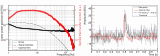
\includegraphics[scale=1]{Figures/ElectrodesExperimental/of_illustration.pdf}
\caption{Illustrations of the Optimal Filtering applied to the heat channel of the detector RED20 taken from the paper [ref]. On the left are displayed the hourly-averaged noise Power Spectral Densities (PSD) (black curves), detector signal bandwidth (black dashed line), and resulting optimal filter transfer functions (red
curves) as a function of frequency, for the six days of data acquisition. The 137 separate PSDs
and transfer functions are overlayed. On the right is an unfiltered raw trace
(grey solid line) and output of the optimal filter (red solid line). The trigger level at $3\sigma$ is shown
as the blue dotted line. The result of the pulse fitting procedure, with a $\chi^2/\textsf{ndf} = 1.03$, is shown
as the black long-dashed line.}
\label{fig:optimal-filtering}
\end{figure}

The noise PSDs $J_{CH}(f)$ of the heat and ionization channels are determined experimentally each hour with samples of \SI{1}{\s} time traces without pulses. These so-called "noise events" are uniformly selected at random throughout the entire data stream on that hour. The signal functions $s_{CH}(t)$ corresponds the signal templates \ref{eq:heat-channel-signal-function} for the heat channel and \ref{eq:ionization-channel-signl-function} for the ionization channels. The hourly heat noise LPSDs and signal power spectrum associated with RED20, corrected for the 2 Hz filter gain, are overlaid on the left subplot of figure \ref{fig:optimal-filtering}.

For each channel $CH$ and for each hour, an optimal filter function $H_{CH}(f)$ is derived from the noise PSD $J_{CH}(f)$ and the conjugate of the signal Fourier transform $\hat{s}^*_{CH}(f)$ such that:
\begin{equation}
\label{eq:optimal-filter}
H_{CH}(f_i) = 
h \cdot \frac{\hat{s}_{CH}^*(f_i)}{J_{CH}(f_i)}
\cdot e^{-i 2 \pi f_i t^M}
\quad \textsf{with} \quad
h =
\left( \sum_i
\frac{|\hat{s}_{CH}(f_i)|^2}{J_{CH}(f_i)}
 \right)^{-1}
\end{equation}
with $t^M$ is the time position of the pulse template maximum and the frequencies $f_i \in [-f_s/2\, .. \,f_s/2]$. The term $h$ is a normalization constant that preserves the amplitude of the pulse signal. The moduli $|H_{heat}(f_i)|$ associated with RED20 are shown as the red solid lines in the left panel of figure \ref{fig:optimal-filtering}. This plot confirms that the optimal filter gives more weight to frequencies with high signal-to-noise ratio. The optimal filters are applied to the five heat and ionization channels of the data stream.

% trigger
The trigger step of the processing consists in identifying candidate pulses in the filtered data stream as an event. An event is a time window of length $T_{win.} = \SI{0.5}{\s}$ from a data stream. A triggering event is defined when a filtered channel exceed a given threshold level $A_{CH}^{trig.}$. The event is centered on the local maximum of the OF filtered data stream passing this amplitude threshold. The instances when multiples such local maxima are identified within the same \SI{0.5}{\s} time windows are called "pile-up" events. In this cases, only one event is defined centered on the pulse with the highest amplitude, imposing an exclusion interval of $\pm\SI{0.25}{\s}$ where the lowest pulses cannot trigger.
This energy ordering of the pulse finding algorithm affects the energy dependence of the triggering efficiency. For instance, the dead-time associated to the search
for low-energy events is effectively greater than that associated to large pulses which are favored in the triggering process. A dedicated data-driven procedure, the pulse simulation presented in the paragraph \ref{par:pulse-simulation}, is applied to take into account these effects in the determination of the efficiency as a function of energy. 

The right subplot of the figure \ref{fig:optimal-filtering} displays a triggering event. It compares the raw heat pulse and its OF filtered version. The amplitude threshold $A_{CH}^{trig.}$ is represented by the horizontal line. The threshold level is defined as a fixed number $n$ of the baseline energy resolution $\sigma_{CH}^{OF}$. This resolution corresponds to the standard deviation of the amplitudes of the noise events.
The value of $n$ was chosen such that the rate of noise induced triggers is significantly smaller than the rate of physical events, which is about \SI{1}{\Hz}. In this analysis, the trigger threshold is set to $A_{CH}^{trig.} = 3 \cdot \sigma_{CH}^{OF}$. For the default polarization of the detector RED80, the trigger thresholds are in average:
\begin{equation}
\begin{cases}
A_{heat}^{trig.} \approx 3 \times \SI{9}{\textsf{ADU}} = \SI{27}{\textsf{ADU}} = \SI{240}{\eV} \\
\forall X \in \{A,B,C,D \}, 
A_{X}^{trig.} \approx 3 \times \SI{1.3}{\textsf{ADU}} = \SI{3.9}{\textsf{ADU}} = \SI{735}{\eV}
\end{cases}
\end{equation}
A pulse can trigger with either its heat or ionization signals. However, due to the low heat resolutions, most events trigger with the heat channel especially at the lowest recoil energies.



% event processing
Each triggering event is further processed to estimate its amplitude. Each channel $CH$ is adjusted by the corresponding signal models, in equation \ref{eq:heat-channel-signal-function} for the heat channel and equation \ref{eq:ionization-channel-signl-function} for the ionization channels. The model adjustment is done by minimizing a $\chi^2$ function defined in the frequency domain:
\begin{equation}
\chi_{CH}^2(a, t) =
\sum_i 
\frac{
|\hat{V}_{CH}(f_i) - a \cdot \hat{s}_{CH}(f_i) \cdot e^{-i 2 \pi f_i t}|^2
}{
J_{CH}(f_i)
}
\end{equation}
where $a$ corresponds to the scaling factor of the unitary signal template and $t$ is the starting time of the pulse. Considering the number of points composing an event, each $\chi^2$ functions should tend to $200$. The minimization yields several quantities. First, the minimal $\chi^2$ value of the event the minimizing amplitude which quantifies the quality of the fit. This value is used to enforce the $\chi^2$ cut described in the next paragraph \ref{par:quality-cuts}. Then, the minimizing parameters $a$ and $t$. The amplitude $a$ is an estimation of the amplitude $A_{CH}$ of the signal. The five amplitudes of the heat and ionization channel are used to reconstruct the heat $E_{heat}$ and ionization $E_{Ion.}$ energies. Eventually this leads to estimate the recoil energy $E_R$ deposited in the germanium crystal by an interacting particle. The time $t=t^0$, called the timestamp of the event, corresponds to the location of the event within the data stream. It is used to monitor the performances of the detector over time and define the live time in paragraph \ref{par:live-time-cut}. Moreover, the timestamp of an event is compared to the maintenance period and the reset times of a detector as part of the quality cuts in paragraph \ref{par:quality-cuts}.


% Heat Offset
Another quantity can be extracted from the raw signals. The offset corresponds to the baseline of an event inside the ADU dynamic range. In the case of the heat channel, the heat offset is a linear function of the resistivity of the NTD thermal sensor. By monitoring the heat offset, we can access the temperature of the detector $T_{abs} \approx T_{NTD}$. If represented as a function of the timestamp $t_0$, it is possible to check on the stability of the detector thermalization which is used to define the live time cut in paragraph \ref{par:live-time-cut}.
% Ionization Offset
For the ionization channel, the offsets of all the electrodes are periodically set to \SI{0}{\textsf{ADU}} by the reset procedure described in the paragraph \ref{par:reset-procedure} as not to leave the dynamic range of the acquisition electronics. The ionization offset is further discussed in the next paragraph \ref{par:quality-cuts} as to define the "offset cut".

% Ionization Slope [Bonus]
% Slope Ionization vs Timestamp: this curve is proportional to the baseline current measured by each electrodes. This baseline current is explained by the presence of leakage current between the electrodes (dedicated section?) and the collection of trapped charges (especially after a maintenance).


\subsection{Live Time Cut}
\label{par:live-time-cut}

%%% blabla
%{\color{red} Need to link this to the window length of 1s. Because a shorter window length would increase the livetime at the cost of the resolution i think.}
%
%The raw streams have various "fine" time intervals where the data can be taken properly. These fine intervals define the so-called "Livetime cut" which discarded any events not in the fine intervals. In the figure \ref{fig:analysis-monitoring-demo}, all the events are plotted in gray while only the events passing the Livetime cut are plotted in blue. The intervals were chosen with some precautionary buffer in to apply a conservative cut that would reject any abnormal event. In the end, the livetime is obtained for each streams and added for both configuration, giving a livetime of $75.6$ hours for the Calibration and $35.93$ hours for the Background.
%
%It appears that RED80 was operated at a constant temperature for the duration of this stream (this is also observed for all the other streams). Indeed, the events corresponding to the calibration peaks are reconstructed with a fixed amplitude (approximately $2 \times 10^2$ ADU for the 1.3keV and $2 \times 10^3$ ADU for the 10.37keV), and thus we check that the sensitivity of the heat channel is constant for the whole stream.
%
%However, some strange periods of time are visible where no events were saved. In the presented figure, it is most notable in the intervals $[7, 11.3]$ and $[13.8, 14.1]$ hours. 

The live time $T_{live}$ corresponds to the period of time where the detector is considered available for data taking. While we would like the live time to equal the whole running time of the detector, it is often not the case. There can be some periods where the temperature regulation of the cryostat can be defective (temperature spikes, power cuts) which degrade the heat sensitivity of the detector. These periods are pruned as to keep only the data with optimal operation of the detectors. Some periods are affected various malfunctions not clearly understood relative to the acquisition electronics. These portions of the streams were corrupted with no data saved all together. During this time, the detector is not considered to be live. The live time are manually defined by monitoring all the control values defined in the previous paragraph \ref{par:data-format} as functions of the timestamp.

Although a high live time is linked with a high events statistics, the estimation of $T_{live}$ is used in the calculation of the exposure of the detector. This exposure is discussed later in the paragraph \ref{par:exposure} when presenting the results of the IP2I neutron background measurement. Indeed, this exposure is used to normalized the counts as to derived the event rate. The live times associated the RED80 streams for the neutron study are listed in the table \ref{tab:neutron-live-time} in the next chapter \ref{ChapterNeutron}.
%It is important to consider the appropriate live time for a stream as all the results presented in the analysis will eventually be weighted by the exposure of the detector and so this very live time. 

In the present paragraph, the results are not normalized by the exposure, and the live times are of minimal importance. As such for the RED80 and REDN1 data streams used for the comparison to electrostatics simulation, the live time is considered to be the length of the data stream of an average of 2 hours. As such, for all the streams listed in tables \ref{tab:red80-stream-list} and \ref{tab:redn1-stream-list}, all the events pass the live time cut.


\subsection{Quality Cuts}
\label{par:quality-cuts}

%%% blabla
% Among those triggering events are events of interest well reconstructed and induced by electronic recoil from the radioactive gamma background, the KLM activation lines from the germanium and the cosmic muons and neutron recoil from the AmBe neutron source and the radioactive neutron background. However, many triggering events can not be reconstructed or were induced by parasitic source, and can not yield information for the measurement of the neutron background at IP2I. To extract the events of interest from all the data, analysis cuts are applied.

The objective of the "Quality cuts" is to discard any event with problematic characteristics which would result in an incorrect energy reconstruction. The term "Quality cuts" refers to an ensemble of analysis cuts: the live time cut (described in the previous paragraph), the maintenance cut, the reset cut, the offset cut and the $\chi^2$ cut. Events passing all these quality cuts are designated as "quality events". In addition to the description of each of the quality cuts, this paragraph presents the parametrization specific to the data streams listed in the tables \ref{tab:red80-stream-list} for RED80 and \ref{tab:redn1-stream-list} for REDN1. The parametrization of the quality cuts for the IP2I neutron measurement is presented in the next chapter \ref{ChapterNeutron}.

%% Livestream cut
%The live stream cut described in paragraph \ref{par:livestream-cut} is not applied in this chapter. Indeed, the comparison of the simulation of RED80 and REDN1 to the experiment is not based on the rate of events. As to ease the workload of analysis, this cut is not applied.


% maintenance cut
% reset cut
The maintenance and reset procedures are introduced in the paragraph \ref{par:ionization-electronics}.  The objective of the maintenance is to recharge the electrodes in order to enforce a constant voltage bias on the whole stream. The reset procedures prevents the digital readout of the ionization channels from saturating. Both procedures periodically induce parasite signals in the data streams. Although these electronics artifacts could be easily discarded due to their shape differing from the expected heat and ionization signals, this is no more the case for signals of low energies. Such events could be considered as a valid signal and bias the science results. Therefore, these signals are reliably rejected using the knowledge on the frequency and duration of the maintenance and reset procedures within a data stream.

The "Maintenance cut" enforces that all the event with a timestamp $t_0$ within a maintenance period is discard. In this work, a maintenance last $\SI{1}{\minute}=\SI{60}{\s}$ and occurs every $\SI{864}{\s}\approx\SI{14.2}{\minute}$. In the end, the maintenance procedure induce a down time rate of $60/(60+864)=\SI{6.6}{\percent}$. An event passes the maintenance cut if it does not occurs during a maintenance.

Contrary to the maintenance, a reset is almost instantaneous, generating a single artifact pulse. Consequently, the "Reset cut" rejects events occurring shortly after each reset procedure. As the detectors are operated in above ground conditions, the event rate is high which calls for the very low period of reset $T_{reset} = \SI{2}{\s}$. An event of timestamp $t^0$ passes the reset cut is the time elapsed since the last reset procedure at $t(\textsf{last reset})$ is greater than a tolerance:
\begin{equation}
t(\textsf{last reset}) - t^0 > \Delta t_{tol}=\SI{5}{\milli\s}
\end{equation}
Even if the artifact pulses generated by the resets are discarded in the analysis, they can still overlap with neighboring valid pulses thus creating pile-ups. These pile-ups events are generally rejected in the $\chi^2$ cut.


% Offset Cut
The need for an "offset cut" originates from a dysfunction of ionization readout electronics. The gain applied to the measured signal $V_X$ depends on the ionization offset value. This behavior is consider as faulty as we expect the electrodes to have a constant sensitivity. This phenomenon is illustrated in the figure \ref{fig:offset-problem} which plots the ionization amplitude $A_D$ of triggering events as a function of their offset values. For low offsets, the \SI{10.37}{\kilo\eV} calibration events form a band of events of amplitude $A_{D} \approx \SI{55}{\textsf{ADU}}$. However, at the offset value $\SI{23000}{\textsf{ADU}}$, these calibration events are processed with a suddenly lower amplitude of about $\SI{30}{\textsf{ADU}}$. This observation is common to all the electrodes $X \in \{ A,B,C,D \}$. We can conclude that the gain of the electronics is constant before $\SI{23000}{\textsf{ADU}}$ and almost halved after. As such, only a part of the readout dynamic range ensures an optimal operation of the detector. Applying a significant safety buffer, the valid dynamic range is $[-14000, +14000]\ \textsf{ADU}$. Events occurring with half gain are discarded by the offset cut, which is illustrated on the figure \ref{fig:offset-problem} by the red region.

\begin{figure}
\centering
\includegraphics[scale=1]{Figures/ElectrodesExperimental/offset_cut.png}
\caption{Graph of the amplitude $A_{D}$ of the triggering events of the data stream tg18l005 for detector RED80 versus their offset value. The dense population of amplitude $A_{D} \approx \SI{55}{\textsf{ADU}}$ corresponds to the \SI{10.37}{\kilo\eV} calibration events. From $\SI{23000}{\textsf{ADU}}$ in offset, their amplitude drops to about $\SI{30}{\textsf{ADU}}$, demonstrating the  $1/2$ gain loss of the electronics. The red overlay span illustrates the offset cut for the electrode $D$.}
\label{fig:offset-problem}
\end{figure}


% Chi2 Cut
As introduced in the paragraph \ref{par:optimal-filtering} describing the event processing, the $\chi_{CH}^2$ values of an event quantify the quality of the adjustment by the signal template and consequently, the quality of the estimation of the amplitude $A_{CH}$.

\begin{equation}
\mathbb{E}\left( \chi^2 \right)  = \chi_0^2
 = T_{\textsf{window}} \cdot f_s = 200
\end{equation}

Concerning the $\chi^2$ value, the threshold depends on the energy. Indeed, because of non-linearity in the bolometer heat response, the shape of the signal do depends on the recoil energy as the first order perturbation theory becomes less and less valid.
Good events at low energy should have a $\chi^2$ value of about:

The $\chi^2$ value of good events is increasing from $\mathcal{O}(10keV)$.
Therefore, a cut parametrization function depending on the event amplitude is chosen:

\begin{equation}
Threshold(Amplitude) 
= \gamma \times \mathbb{E}\left( \chi^2 \right)  \times \left[ 1+ \left( \frac{Amplitude}{\alpha} \right)^\beta \right]
\end{equation}

with $\alpha$, $\beta$ and $\gamma$ 

All the events with any estimated $\chi^2$, on the heat channel or one of the ionization channels, above a defined threshold function is discarded from the analysis.
The threshold is a function of the signal amplitude $A_X$ of a channel $X$ in ADU. Its expression is
\begin{equation}
\chi_{cut}^2 (A_X) = \chi_0^2 \cdot \left( 1 + \left( \frac{A_X}{A_0} \right)^b \right)
\end{equation}
depending on the three parameters: the baseline threshold $\chi_0^2$, the takeoff amplitude $A_0$ and the quadratic factor $b$. The parameters are estimated visually for each streams and presented in table \ref{tab:red80-redn1-chi2-cut}.

\begin{table}[]
\centering
\begin{tabular}{c|l|c|c|c}
Detector               & Channel & $\chi_0^2$                & $A_0$                      & $b$ \\ \hline \hline
\multirow{3}{*}{RED80} & Heat    & \multirow{2}{*}{400}      & \num{3e3} & 2   \\ \cline{2-2} \cline{4-5} 
 &
  \begin{tabular}[c]{@{}l@{}}Ionization\\ $A,B,C,D$\end{tabular} &
   &
  \multicolumn{1}{r|}{\num{2e3}} &
  \multicolumn{1}{r}{2.2} \\ \hline
\multirow{3}{*}{REDN1}                  & Heat    & \multicolumn{1}{r|}{2000} & \num{3e3} & 2   \\ \cline{2-3} \cline{4-5} 
 &
  \begin{tabular}[c]{@{}l@{}}Ionization\\ $A,B,C,D$\end{tabular} &
  \multicolumn{1}{r|}{700} &
  \multicolumn{1}{r|}{\num{2e3}} &
  \multicolumn{1}{r}{2.2}
\end{tabular}%
\caption{Parametrization of the $\chi^2$ cut for the data streams listed in tables \ref{tab:red80-stream-list} and \ref{tab:redn1-stream-list} for the detectors RED80 and REDN1 respectively.}
\label{tab:red80-redn1-chi2-cut}
\end{table}

In the end, the $\chi^2$ cut is applied on each channels (as seen in figure \ref{fig:chi2-cut}) independently. Only the events passing the cut for all the channels is kept and eligible as a quality event.

\begin{figure}
\centering
\includegraphics[width=\linewidth,]{Figures/ElectrodesExperimental/chi2_cut.png}
\caption{$\chi^2$ value for each event in function of its reconstructed amplitude for the five measuring channels. The cut threshold is represented by the black line. All events are in red, passing events are in blue.}
\label{fig:chi2-cut}
\end{figure}


\subsection{Cross-talk correction and Cabling capacitance estimation}

The paragraph \ref{par:sensitivity-calculation} discuss the expression of the signal induced on the ionization channel by a recoil. It is demonstrated that a recoil, creating a number $N_p$ of electron-hole pairs, generates a charge perturbation on the electrodes $A$ through $D$. This perturbation is expressed as the charge perturbation vector $\vec{Q}$. In the case of the REDN1 and RED80, there are different charge perturbation vector depending on the recoil location in the crystal. Their expression are displayed in equation \ref{eq:red80-induced-charges} for RED80 and \ref{eq:fid38-induced-charges} for REDN1, considering an ideal drift of the charges and a complete collection on the electrodes.
The voltage signal $\vec{V}$ generated on the electrode is calculated from the charge vectors and the Maxwell capacitance matrix $C$ of the detector according to the equation \ref{eq:capacitance-definition-matrix}. It is calculated in the equations \ref{eq:planar38-sensitivity} for the PL38 design and the equations \ref{eq:fid38-sensitivity} for the FID38 design. Contrary to the charge vector $\vec{Q}$ which has 2 null component, a voltage signal is generated on all the electrodes of the detector. This phenomenon is called cross-talk.
The cross-talk correction is an analysis step consisting in calculating an effective charge vector $\vec{Q}_{eff}$ from the amplitude $A_{CH}$ of the measured ionization voltage signals, corresponding to the measured voltage vector $\vec{V}_{meas.}$. With cross-talk corrected measurement, it is possible to proceed with the calibration of the detector and the rest of the analysis.
The calculation is done with the cross-talk correction matrix $\bm{C}_{X-talk}$ such that:
\begin{equation}
\label{fig:cross-talk-correction}
\vec{Q}_{eff} = \bm{C}_{X-talk} \cdot \vec{V}_{meas.} =
\bm{C}_{X-talk} \cdot
\begin{pmatrix}
A_A \\ A_B \\ A_C \\ A_D
\end{pmatrix}
\end{equation}
with the terms $A_X^{corr.}$ being the cross-talk corrected amplitudes in ADU.
This equation is the experimental equivalent of the equation \ref{eq:capacitance-definition-matrix} dedicated to theoretical perturbation vector $\vec{Q}$ and $\vec{V}$ on a detector of known Maxwell capacitance matrix $\bm{C}$. As a result, the cross-talk correction matrix is equal to the Maxwell capacitance matrix of the detector and the cabling such that:
\begin{equation}
\bm{C}_{X-talk} = \bm{C}_{total} = \bm{C}_{detector} + \bm{C}_{cabling} 
\end{equation}
The Maxwell capacitance matrix of the detector $\bm{C}_{detector}$ is considered known as it is yielded from the detector simulation in the equations \ref{eq:red80-maxwell} and \ref{eq:redn1-maxwell} for RED80 and REDN1 respectively.
The paragraph \ref{par:sensitivity-calculation} explains that the cabling possesses a diagonal Maxwell capacitance matrix. Under the assumption that the properties of the cabling, like its length or its shielding, is the same for all the electrodes, all its diagonal components are equals. Their value is a single cabling capacitance $C_{cabling}$ which is unknown.
Therefore, all the non-diagonal terms of the cross-talk correction $C_{X-talk}$ matrix are known and its diagonal terms are to be defined through the estimation of the cabling capacitance $C_{cabling}$.

This estimation is based on the ionization signatures of the events expected from the fully collected bulk, guard or veto events induced by the \SI{10.37}{\kilo\eV} calibration electronic recoils. This estimation process is therefore iterative as cross-talk correction and energy calibration are interdependent. 
For this analysis, the cross-talk correction is first approximated with a graphical method. The calculated effective charge signal $\vec{Q}_{eff}$ are then used in the calibration step, described in the following paragraph \ref{par:calibration-step}, and in the selection of the calibration events described in the paragraph \ref{par:calibration-events-selection}. The precise cross-talk correction is done with the \SI{10.37}{\kilo\eV} calibration events only and the analysis pipeline is re-run with this additional precision.

% Graphical method
The cross-talk correction matrix $\bm{C}_{X-talk}$ and more specifically the cabling capacitance $C_{cabling}$, are approximated with a graphical method. The principle is to have the effective charge perturbation vector $\vec{Q}_{eff}$ correspond to the theoretical charge perturbation vectors $Q$ for the different collection volume: bulk, guard, veto as expressed in equations \ref{eq:red80-induced-charges} and \ref{eq:redn1-induced-charges}. As the detector is not calibrated yet, the component of the theoretical charge vector are known up to a calibration factor $a_X$ depending on the electrode $X$. Considering the bulk events of RED80 as reference, the equation that is solved graphically with $C_{cabling}$ as unknown is the following:
\begin{equation}
\label{eq:crosstalk-correction}
\begin{bmatrix}
a_A & 0 & 0 & 0 \\
0 & a_B & 0 & 0 \\
0 & 0 & a_C & 0 \\
0 & 0 & 0 & a_D \\
\end{bmatrix}
\cdot
\vec{Q}_{bulk}
=
\begin{bmatrix}
0 \\ -a_B \\ 0 \\ a_D
\end{bmatrix} 
=
\left( \bm{C}_{detector} + C_{cabling} \cdot \mathbb{1} \right) \cdot \vec{V}_{meas.}(\textsf{Bulk events})
\end{equation}

As the calibration coefficient $a_X$ are unknown, it is handy to consider a normalized cross-talk corrected signal vector $\vec{Y}$ expressed as:
\begin{equation}
\begin{split}
\vec{Y}^{bulk}
&=
\frac{1}{C_{detector, 11} + C_{cabling}}
\left( \bm{C}_{detector} + C_{cabling} \cdot \mathbb{1} \right) \cdot \vec{V}_{meas.}(\textsf{Bulk events})
\\
&= C_{X-talk}^N \cdot \vec{V}_{meas.}(\textsf{Bulk events})
\end{split}
\end{equation}
with $\bm{C}_{X-talk}^N$ the normalized cross-talk correction matrix.

With a correctly estimated $C_{cabling}$ satisfying the equation \ref{eq:crosstalk-correction}, the cross-talk corrected signal vector $\vec{Y}^{bulk}$ of the bulk event has two null components $Y_A^{bulk} = Y_C^{bulk} = 0$ and two non-null components $Y_B^{bulk}$ and $Y_D^{bulk}$.
In order to visualize the four components of the cross-talk corrected vector $\vec{Y}$ visualization, corner plots are used . The figure \ref{fig:red80-crosstalk-correction} present such a corner plot for the detector RED80 for the stream tg09l000 in the Run 57. Only events passing the quality cuts are plotted. The dashed guide lines indicates the null signal at \SI{0}{ADU} and the full collection of the \SI{10.37}{\kilo\eV} calibration electronic recoils  at $\approx \pm \SI{55}{ADU}$ (drawn a fortiori after the calibration step).
Each color corresponds to a different cabling capacitance value $C_{cabling}$ with the vector $\vec{Y}(\SI{125}{\pico\farad})$ colored in orange, $\vec{Y}(\SI{0}{\pico\farad})$ colored in green and $\vec{Y}(+\infty)$ colored in blue. We note that as $C_{cabling} \rightarrow +\infty, \ \bm{C}_{X-talk}^N \rightarrow \mathbb{1}$. The non-diagonal terms of the normalized cross-talk correction matrix $\bm{C}_{X-talk}^N$ are inversely proportional to the cabling capacitance $C_{cabling}$. As a result, we observe a diminishing return in the change of shape of the vector $\vec{Y}$ with increasing $C_{cabling}$.

\begin{figure}
\centering
\includegraphics[scale=1]{Figures/ElectrodesExperimental/red80_crosstalk_correction.png}
\caption{Corner plot of the cross-talk corrected amplitude vector $\vec{Y}$ in ADU. The plotted events belong corresponds to the stream tg09l000 of the run 57 operating the detector RED80. Only events passing the quality cuts are displayed. Each color corresponds do a different cabling capacitance $C_{cabling}$ used to calculate the cross-talk correction matrix $\bm{C}_{X-talk}$. The guide lines indicate no collection at \SI{0}{ADU} and full collection at $\approx \pm \SI{55}{ADU}$ of the \SI{10.37}{\kilo\eV} calibration electronic recoils.}
\label{fig:red80-crosstalk-correction}
\end{figure}

The correct cabling capacitance $C_{cabling}$ satisfying the equation \ref{eq:crosstalk-correction} is chosen when the distribution of the components of $\vec{Y}$ in the corner plots mostly corresponds to the guide lines.
In the case of $RED80$ and $REDN1$, the cabling capacitance was first estimated to $C_{cabling} = \SI{120}{\pico\farad}$. 
We  can check that the normalized cross-talk correction matrix $\bm{C}_{X-talk}^N$ corresponds to the identity matrix at the first order. The correction terms are in the range of few percents, going up to $5.2\%$ in the case of the case of the electrode $B$ inducing signal on the electrode $A$.

% Precise estimation
The precise estimation of the cabling capacitance $C_{cabling}$ and the cross-talk correction matrix $\bm{C}_{X-talk}$ happens after the calibration step and the selection of the full collected bulk events created by the \SI{10.37}{\kilo\eV} calibration electronic recoils.
A fiducial recoil leads to the induced charge vector:
\begin{equation}
\vec{Q}_{fid}^{REDN1} =ur C
\begin{bmatrix}
0 \\ -1 \\ 0 \\ 1
\end{bmatrix}
\cdot Q(\SI{10.37}{\kilo\eV})
\end{equation}
with the electric charge multiplicative factor being:
\begin{equation}
Q(\SI{10.37}{\kilo\eV})
=
N_p(\SI{10.37}{\kilo\eV}) \cdot e
=
\frac{E_R}{\epsilon} e
=
\frac{\SI{10.37e3}{\eV}}{\SI{2.97}{\eV}} e
\end{equation}

According to equation \ref{eq:matrix-capacitance-charge}, the voltage signal induced on the electrodes is expressed by the vector $\vec{V}_{fid}^{REDN1}$ obtained with the Maxwell capacitance matrix  of the detector and cabling $\bm{C}_{total} = \bm{C}_{detector} + \bm{C}_{cabling}$ such that:
\begin{equation}
\label{eq:redn1-bulk-voltage-vector}
\vec{V}_{fid}^{REDN1}
=
\begin{bmatrix}
V_A \\ V_B \\ V_C \\ V_D
\end{bmatrix}
=
\bm{C}_{total}
\cdot
\vec{Q}_{fid}^{REDN1}
\end{equation}

In the paragraph \ref{par:sensitivity-calculation}, the Maxwell capacitance matrix associated with the cabling $C_{cabling}$ is considered to be diagonal with $\forall i \neq j, \bm{C}_{cabling, ij} = 0$ . The previous equation \ref{eq:redn1-bulk-voltage-vector} can be translated for the terms $V_i$ and $Q_i$ of the vectors $\vec{V}_{fid}^{REDN1}=\vec{V}$ and $\vec{Q}_{fid}^{REDN1}=\vec{Q}$ respectively:
\begin{equation}
\begin{split}
V_{i}
&=
\sum_{j=1}^4 C_{total, ij} Q_j
\\
&=
\sum_{j=1}^4 C_{detector, ij} Q_j + \sum_{j=1}^4 C_{cabling, ij} Q_j
\\
&=
\left(
 C_{detector, i4} - C_{detector, i2}
\right)
Q(\SI{10.37}{\kilo\eV}) + C_{cabling, ii} Q_i
\end{split}
\end{equation}

We assume that the Maxwell capacitance matrix relative to the detector $\bm{C}_{detector}$ is known as it calculated from the electrostatics simulation of REDN1. The diagonal terms $\bm{C}_{cabling, ii}$ of the cabling capacitance matrix can therefore be evaluated from the voltage signal induced by the \SI{10.37}{\kilo\eV} fiducial events $\bm{V}_{i}$ :
\begin{equation}
\label{eq:cabling-capacitance-expression}
C_{cabling, ii}
=
\frac{1}{Q_i} \left[ \bm{V}_{i} - \left( C_{detector, i4} - C_{detector, i2} \right) Q(\SI{10.37}{\kilo\eV}) \right]
\end{equation}

One should note that as $Q_1 = Q_3 = 0$, the equation \ref{eq:cabling-capacitance-expression} is only valid for $i \in \{ 2,4 \}$. This means that the fiducial events collected by the electrode $B$ and $D$ can only be used to determine the cabling capacitance associated with these very electrodes $C_{cabling, 22}$ and $C_{cabling, 44}$ respectively. A precise estimation of the cabling capacitances affecting the electrodes $A$ and $C$ would necessitate to adjust the veto or guard events which lack statistics.

The figures \ref{fig:red80-cabling-capacitance} and \ref{fig:redn1-cabling-capacitance} displays the histograms derived from the values $C_{cabling, 22}$ and $C_{cabling, 44}$ computed with the equation \ref{eq:cabling-capacitance-expression} for each of the \SI{10.37}{\kilo\eV} calibration events passing the Bulk cut for the detectors RED80 and REDN1 respectively. The estimation of the cabling capacitances and their associated error bars are extracted from the quantiles 0.16, 0.50 and 0.84 of the distributions:
\begin{align}
C_{cabling, 22}^{RED80} &= 129_{-8}^{+9} \ \si{\pico\farad}
\quad \quad 
& C_{cabling, 44}^{RED80} &= 125_{-8}^{+9} \ \si{\pico\farad}
\\
C_{cabling, 22}^{REDN1} &= 124_{-7}^{+11} \ \si{\pico\farad}
\quad \quad 
& C_{cabling, 44}^{REDN1} &= 125_{-7}^{+10} \ \si{\pico\farad}
\end{align}
All the values are very similar and compatible within their $1\sigma$-error bars. The small differences in cabling capacitance could be explained by small variation in length of the cabling between the conductive tracks on the copper chassis in the suspended tower and the electronics on the fixed mixing chamber of the cryostat.

\begin{figure}
\centering
\includegraphics[scale=1]{Figures/ElectrodesExperimental/red80_cabling_capacitance_fitting.pdf}
\caption{Histogram and CDF derived from the experimental estimation of the cabling capacitance  $C_{cabling, 22}$ and $C_{cabling, 44}$ for each Bulk events in the RED80 detector.}
\label{fig:red80-cabling-capacitance}
\end{figure}

\begin{figure}
\centering
\includegraphics[scale=1]{Figures/ElectrodesExperimental/redn1_cabling_capacitance_fitting.pdf}
\caption{Histogram and CDF derived from the experimental estimation of the cabling capacitance  $C_{cabling, 22}$ and $C_{cabling, 44}$ for each Bulk events in the REDN1 detector.}
\label{fig:redn1-cabling-capacitance}
\end{figure}

In the end, we consider the collect electrodes $B$ and $D$ of both detectors RED80 and REDN1 to be affected by a common cabling capacitance $C_{cabling} = \SI{125}{\pico\farad}$. We extrapolate this estimation to the auxiliary electrodes $A$ and $C$. The decorrelated amplitudes $A_X$ are processed into the cross-talk corrected amplitude $A_X^{corr.}$ according to the equation \ref{eq:crosstalk-correction} using the determined $C_{cabling}=\SI{125}{\pico\farad}$.

In future studies and with enough statistics, we can imagine a more complex and precise cross-talk correction by considering one cabling capacitance term specific to each electrode.


\subsection{Calibration and Selection of the \SI{10.37}{\kilo\eV} Calibration Events}
\label{par:ion-calibration}
\label{par:heat-calibration}
\label{par:10kev-selection}

The five measurements channels are saving the voltage of their associated sensors in ADU unit specific to each considered channel. In order to proceed with the estimation of the heat $E_{heat}$, ionization $E_{Ion.}$ and recoil $E_R$ energies, it is now necessary to determine the conversion rates between ADU units and \si{\eV} for each channel $CH$. This calibration coefficient $\alpha_{CH}$ are determined experimentally thanks to the intrinsic germanium \SI{10.37}{\eV} calibration line inducing electronic recoils of known heat energy $E_{heat} = \SI{10.37}{\kilo\eV_{ee}}$ and ionization energy $E_{Ion.} = \SI{10.37}{\kilo\eV}$. This subsection first describes the calibration of the ionization channel. Then, it discusses the selection of the \SI{10.37}{\kilo\eV} calibration events for the calibration of the heat channel.

The most straightforward calibration method is to determine the position of this calibration peak on the amplitude spectra of the electrodes $A,B,C,D$. Indeed, according to the charge signatures \ref{eq:red80-induced-charges} of the events in the detector RED80, the charge are induced on the two collecting electrodes with equal amplitude. However, due to the oblique propagation of the electrons, a significant fraction of the \SI{10.37}{\kilo\eV} events does not possess these archetypal ionization signature but rather a linear combination. Although this phenomenon affects only slightly the calibration of the collect electrodes $B$ and $D$ due to the high fraction of bulk events with complete charge collection, the low amount of well reconstructed guard events render the precise calibration of the guard electrodes $A$ and $C$ impossible. 

The alternative calibration method, used in this work, permits the precise calibration of all the electrodes by benefiting from the non-ideal ionization signatures being linear combination of the bulk, guard and guard-collect events. The figure \ref{fig:ion-calibration} illustrates this ionization calibration method for the RED80 data streams relative to the neutron background measurement. The graphics plots the cross-talk corrected amplitudes $A_X^{corr.}$ of all the quality events as red points. The left graphics shows that all events produce negative amplitudes on the electrodes $A$ and $B$ which is consistent with the fact that in at the default polarization \ref{eq:red80-default-polarization}, $A$ and $B$ collect electrons. Similarly, the electrode $C$ and $D$ collect holes inducing signals with positive amplitude.

\begin{figure}
\centering
\includegraphics[scale=1]{Figures/ElectrodesExperimental/ion_calibration.png}
\caption{Calibration of the electrodes $A,B,C,D$ of the detector RED80 on the data stream tg18l005. The left graphics displays the amplitude display the cross-talk corrected amplitudes $A_A^{corr.}$ versus $A_B^{corr.}$. Similarly, the right graphics plots $A_C^{corr.}$ versus $A_D^{corr.}$. All the quality events are represented in red. The blue events corresponds to \SI{10.37}{\kilo\eV} calibration quality events with complete charge collection. Their amplitudes is adjusted with a linear law yielding the amplitudes $A_X^0$ of the fully collected \SI{10.37}{\kilo\eV} peak.}
\label{fig:ion-calibration}
\end{figure}

The blue points are quality events which are selected with the following conditions:
\begin{equation}
\begin{cases}
A_{heat} > \SI{500}{\textsf{ADU}} \\
\SI{100}{\textsf{ADU}} > |A_{tot}^{corr.}| > \SI{150}{\textsf{ADU}} \\
\textsf{with  } A_{tot}^{corr.} = \frac{1}{2} \left( -A_A^{corr.}-A_B^{corr.}+A_C^{corr.}+A_D^{corr.} \right)
\end{cases}
\end{equation}
with $A_{tot}^{corr.}$ the total ionization amplitude. This selection crudely corresponds to the \SI{10.37}{\kilo\eV} calibration events with a complete charge collection $E_{Ion.} \approx \SI{10.37}{\kilo\eV}$. As the electrons (resp. holes) are collected by both the $A$ and $B$ (resp. C and D) electrodes, the ionization energy $E_{Ion.}$ is split between the two electrodes. The calibration of the electrodes of REDN1 is done using the same method with the difference that the electrons are collected by the electrodes $A,D$ and the holes by $B,C$.

The black lines are linear laws adjusted to the blue population using orthogonal distance regression. The parameters of the linear laws, $A_X^0$, are the positions of the calibration peaks when fully collected by either one of the electrodes. 

The calibration coefficient $\alpha_X$ are defined for each electrodes $X$ as:
\begin{equation}
\alpha_X = \frac{\SI{10.37}{\kilo\eV}}{A_X^0}
\end{equation}

The calibrated amplitudes in \si{\kilo\eV} are called the electrode specific ionization energies $E_X$ and defined as:
\begin{equation}
\forall X \in \{ A, B ,C,D \}, \quad 
E_X = \alpha_X \cdot A_X^{corr.}
\end{equation}
The ionization energy $E_X$ is proportional to the charge $Q_X$ induced on the electrode $X$ and estimates the fraction of the ionization energy $E_{Ion.}$ measured by this electrode. The estimation of the ionization energy $E_{Ion.}$ created by the recoil is the quantity $E_{Ion.}^{tot}$ called the total ionization energy. In its default polarization, the total ionization energy for the detector RED80 is expressed as:
\begin{equation}
E_{Ion.}^{tot} = \frac{-E_A -E_B + E_C + E_D}{2}
\end{equation}
In the case of REDN1 with default polarization, the total ionization energy becomes:
\begin{equation}
E_{Ion.}^{tot} = \frac{E_A - E_B - E_C + E_D}{2}
\end{equation}

The calibration of the heat channel is also based on the \SI{10.37}{\kilo\eV} calibration events. This calibration process is illustrated for the detector RED80 on the stream tg18l005. The figure \ref{heat-calibration} presents the total ionization energy $E_{Ion.}{tot}$ of all the quality events versus their heat amplitude $A_{heat}$.

\begin{figure}
\centering
\includegraphics[width=\linewidth,]{Figures/ElectrodesExperimental/heat_calibration.png}
\caption{Reconstructed Ionization Energy in function of the Reconstructed Heat Energy, for the quality events of the Calibration configuration. The plot is zoomed up to 12keV for an easier view of the calibration peaks. }
\label{fig:heat-calibration}
\end{figure}

Thanks to high rate of calibration events, we easily recognize the band of the \SI{10.37}{\kilo\eV} calibration events. This bands follow a linear law stretched between two remarkable points. The first corresponds to the \SI{10.37}{\kilo\eV} calibration peak, formed by event with a complete charge collection yielding a complete Luke-Neganov boost, located at $A_{heat}\approx \SI{1200}{\textsf{ADU}}$ and $E_{Ion.}^{tot} = \SI{10.37}{\kilo\eV}$. The second point is situated at $A_{heat}\approx \SI{700}{\textsf{ADU}}$ and $E_{Ion.}^{tot} = \SI{0}{\kilo\eV}$. It corresponds to \SI{10.37}{\kilo\eV} calibration events with no charge collection: the electron-hole pairs recombine immediately after the recoil and there is no Luke-Neganov boost on the heat channel. All the calibration events between these points have an incomplete charge collection with only a partial Luke-Neganov boost.

The blue events on the figure corresponds to the manual selection of the calibration events. This selection is made manually with a graphical lasso selection. All the events of these selection are designated in the analysis as "calibration events" and their are used to determine precisely the heat amplitudes of the two extreme points of the calibration bands. The  amplitude of the completely collected calibration peak is $A_{heat}^{peak}$. The heat amplitude of the calibration events with no charge collection is  $A_{heat}^{HO}$. The exponent $HO$ refers to "Heat-Only", as these events do not induce any ionization signal. The selection of calibration events are adjusted with the linear law:
\begin{equation}
E_{Ion.}^{tot} = \frac{10.37}{A_{heat}^{peak} - A_{heat}^{HO}} (A_{heat} - A_{heat}^{HO})
\end{equation}
using an orthogonal distance regression algorithm. The calibration coefficient $\alpha_{heat}$ associated with the heat channel is calculated as:
\begin{equation}
\alpha_{heat} = \frac{\SI{10.37}{\kilo\eV_{ee}}}{A_{heat}^{peak}}
\end{equation}
The calibrated heat amplitude called the heat energy of an event is defined as:
\begin{equation}
E_{heat} = \alpha_{heat} \cdot A_{heat}
\end{equation}
This heat energy is expressed in the unit $\si{\kilo\eV_{ee}}$ where the index $ee$ refers to the "electronic recoil". This unit expresses the heat energy $E_{heat}$ generated by an electronic recoil of quenching factor $Q_{ER}=1$ and recoil energy $E_R$ according to the equation \ref{eq:heat-energy-nl-boost}:
\begin{equation}
E_{heat} = E_R \cdot \left( 1 + \frac{V_{bias}}{2.97} \right)
\end{equation}
As such, the heat calibration assumes that every event is induce by an electronic recoil, which is false in the case of neutron recoils with a lower quenching $Q_{NR}$. This means that apart from the electronic recoils, this experimental heat energy $E_{heat}$ has no physical meaning. However, it is used to access the recoil energy $E_R$ of an event expressed in \si{\kilo\eV}. This recoil energy $E_R$ takes into account the experimental quenching factor of an event $Q$ and the Luke-Neganov Boost $E_{NL}$ associated . 

Combining the equations \ref{eq:quenching} and \ref{eq:nl-energy-simple}, the Luke-Neganov energy of an event is derived from the ionization energy as:
\begin{equation}
E_{NL} = E_{Ion.}^{tot} \frac{V_{bias}}{2.97}
\end{equation}
The recoil energy $E_R$ of an event is calculated as:
\begin{equation}
E_R = E_C \cdot \left( 1 + \frac{V_{bias}}{2.97} \right) - E_{NL}
= E_C \cdot \left( 1 + \frac{V_{bias}}{2.97} \right) - E_{Ion.}^{tot} \frac{V_{bias}}{2.97}
\end{equation}
and the associated quenching factor is derived using the usual formula \ref{eq:quenching} with experimental estimation:
\begin{equation}
Q = \frac{E_{Ion.}^{tot}}{E_R}
\end{equation}

%%% I dont even
%For this purpose, we use the activation of the KLM lines of the Germanium crystal, which emits a gamma of energy 100eV, 1.3keV and 10.37keV respectively [\cite{germanium-decay}]. This gammas of known energy produce electronic recoils depositing a known energy in the ionization channels and the heat channel, with the latter being boosted with the Luke-Neganov effect [\cite{luke-neganov-effect} and \citep{luke-neganov-interpretation}]. As the quenching of the electronic recoil is different from the one of the nuclear recoil, we use the $keV_{ee}$ which precise that the energy deposit done with an electronic recoil.

%We recognize the noise blob near the origin corresponding to recoils of very low energy and triggering noise windows. Expanding from this noise blob, we note two bands. 
%The electronic recoil band corresponds to events depositing the same energy in the ionization channel and the heat energy channel (both in keVee). They are characterized by a quenching factor of 1. As a matter of fact, the gamma recoil of 1.3keV and 10.37keV coming from the calibration peaks of the germanium belongs to this band. Any event below this band deposited less energy in the ionization channel than in the heat channel, and therefore possess a quenching factor inferior to one. We see that the population blob associated to the 10.37keV is smeared to lower quenching factor. This is due to events of the calibration peaks with incomplete charge collection. We note that this population is following a linear trend, which can be explained by an incomplete Luke-Neganov Boost of the heat channel according to the equation:
%\begin{equation}
%E_{heat} = 6 \textsf{keVee} + \epsilon \frac{2 \textsf{V}}{\epsilon_{Ge}} E_{ion.}
%\end{equation}
%The other major population of events below the electronic recoil band counts a lot of events in the case of the Calibration configuration. This hints that this band corresponds to the nuclear recoil induced by the AmBe neutron source.
%The presence of the two bands in this plot demonstrate the discriminating ability of the associated heat and ionization channels. Note that, although the bands are well separated at high energy, they are merging at low energy due to their width which is fixed by the energy resolution of the heat and ionization channel.

%We recognize the electronic band, centered around $Q=1$ and the nuclear recoil band with $Q<0.4$. We also note some inter-band events like the smearing of the 10.37keV events hinting at the incomplete charge collection.

%HEAT ONLY EVENT
%However, there are some interesting events with a quenching factor $Q=0$ which are known as "Heat-only" events. This population is infamously known in domains in the EDELWEISS experiment [ref?] and CRESST [ref?]. This population could correspond to events with no charge collection, but this is not compatible with the lower count of inter-band events with an incomplete charge collection. An other and more realistic explanation would be the existence of energy deposit in the crystal without ionization. The source of this Heat-only event is still under investigation [ref?].
%
%The merging phenomenon of the bands at low energy is also more visible in this graph with the change of variable. We can even visually witness that the lower part of the 1.3keV event blob is leaking into the higher part of the nuclear band.


\subsection{Charge Conservation Cut}
\label{par:charge-conservation-cut}

The charge conservation cut aims at discarding events which does not respect the charge conservation. Indeed, some events might demonstrate charge collection issue. Drifting charges can be trapped in the germanium and may not end up being collected. In the paragraph \ref{par:ion-calibration}, the ionization energies $E_X$ are proportional to the charges collected on the electrodes of the detector. We define the energy of charge conversation $E_{CC}$ as:
\begin{equation}
E_{CC} = \frac{1}{2} \left( E_A + E_B + E_C + E_D \right)
\end{equation}
By construction, this quantity is proportional to the excess or lack of total induced charges on the electrodes of the detector. Contrary to the total ionization energy $E_{Ion.}^{tot}$, this quantity is common to RED80 and REDN1  as it is independent from the polarization of the electrodes.

As a recoil produces electron-hole pairs, the total electric charge carried by the drifting particles in the crystal should be zero as well as the total collected charges. This is characterized by a the normal distribution of the $E_{CC}$ around zero with a standard deviation $\sigma(E_{CC})$ depending with the recoil energy. In order to apply the cahrge conservation cut, the resolution $\sigma(E_{CC})$ is modeled as a linear function of the heat energy $E_{heat}$:
\begin{equation}
\sigma(E_{CC})(E_{heat})
=
\sigma(E_{CC})(\SI{0}{\kilo\eV}) + \frac{\sigma(E_{CC})(\SI{10.37}{\kilo\eV})}{\sigma(E_{CC})(\SI{0}{\kilo\eV})} \cdot E_{heat}
\end{equation}
with $\sigma(E_{CC})(\SI{0}{\kilo\eV})$ evaluated on the noise blob and $\sigma(E_{CC})(\SI{0}{\kilo\eV})$ evaluated on a \SI{0.5}{\kilo\eV} bin centered on \SI{10.37}{\kilo\eV}.
Events not respecting the charge conservation would stand out of the gaussian profile and can be discarded. An event passes the charge conservation cut if its energy of charge conservation $E_{CC}$ is within a $2\sigma$-margin of the null charge:
\begin{equation}
|E_{CC}| < 2 \cdot \sigma(E_{CC})(E_{heat})
\end{equation}
The charge conservation cut is illustrated in the figure \ref{fig:charge-conservation} with the Background data streams of the detector RED80 for the measurement of the IP2I neutron background. The graphic plots the quantity $E_{CC}$ versus the heat energy $E_{heat}$ of all the quality events. The $2\sigma$ margin is delimited by the black curves. The event passing the charge conservation cut are colored blue while the rejected events are red.

\begin{figure}
\centering
\includegraphics[width=\linewidth,]{Figures/Neutron/charge_conservation.png}
\caption{Energy of charge conservation $E_{CC}$ as a function of the heat energy $E_{heat}$ for the quality events of the detector RED80 for Background data streams. Passing events are in blue while discarded events are in red.}
\label{fig:charge-conservation}
\end{figure}

We do not discern any particular population of event which does not conserve the electric charge. The charge conservation cut can therefore be considered as a safety cut eventually pruning rare outlying events.


\subsection{Fiducial Cut}
\label{par:fiducial-cut}

The fiducial cut, also known as bulk cut, aims at selecting the events generated by recoils located in the fiducial volume of the detector. In other words, the fiducial cut discards any event originating from the other collection volume of the detectors RED80 and REDN1. These other collection volumes, in contact with the crystal surface, generates problematic events with hurt the measurements of nuclear recoils.
One major problem comes from the surface trapping phenomenon, inducing an incomplete charge collection. This eventually leads to some electronic recoils being reconstructed with an artificially low quenching and counted as nuclear recoils.
Another issue arise from recoils induced by the natural radioactive background. These recoils, mainly electronic from $\beta$ radiation, are located in the first \si{\micro\meter} of the crystal surface. By discarding the surface events, we effectively lower the electronic background affecting the measurements.

The signature of the bulk recoil in known for RED80 in equation \ref{eq:red80-induced-charges} and REDN1 in equation \ref{eq:fid38-induced-charges}. For both detectors, these bulk recoils generate a signal on the main collecting electrodes $B$ and $D$ only. As such, the fiducial cut identifies events of the bulk region as events which did not deposited any signal on the auxiliary electrodes $A$ or $C$. The tolerance on the signals of $A$ and $C$ is a multiple of their resolution $\sigma(E_A)$ and $\sigma(E_C)$. These resolutions scales with the energy of the recoil and are thus modeled with a linear law adjusted to the baseline resolutions and the resolution on the 
the resolution $\sigma(E_{CC})$ is modeled as a linear function of the heat energy $E_{heat}$:
\begin{equation}
\forall X \in \{A, C \}, \quad 
\sigma(E_{X})(E_{heat})
=
\sigma(E_{X})(\SI{0}{\kilo\eV}) + \frac{\sigma(E_{X})(\SI{10.37}{\kilo\eV})}{\sigma(E_{X})(\SI{0}{\kilo\eV})} \cdot E_{heat}
\end{equation}
Events passing the fiducial cut are designated as fiducial events or bulk events. In this chapter for the electrostatic study of the detector RED80 and REDN1, the bulk events satisfies the system:
\begin{equation}
\begin{cases}
|E_A| < 5 \cdot \sigma(E_A)(E_{heat}) \\
|E_C| < 5 \cdot \sigma(E_C)(E_{heat}) \\
\end{cases}
\end{equation}
with a $5\sigma$ tolerance.

The fiducial cut is illustrated in figure \ref{fig:fiducial-cut} for the data streams of RED80 used in the neutron background measurement. The two subplots presents the ionization energies of the guard electrodes $E_A$ and $E_C$ of all quality events satisfying charge conservation versus the heat energy of the event. As explained in the next chapter, the tolerances of the analysis cut are globally lower. For the fiducial cut, a $2\sigma$ margin is chosen and delimited with the black curves. We can notice, especially near the \SI{1.3}{\kilo\eV} and \SI{10.37}{\kilo\eV} calibration peaks, that a significant fraction of the events, colored red, are discarded. This events are corresponds to the recoils located in the guard, guard-collect and corners volumes of the detector RED80.

\begin{figure}
\centering
\includegraphics[scale=1]{Figures/ElectrodesExperimental/bulk_cut.png}
\caption{Ionization energies $E_A$ and $E_C$ as a function of the heat energy $E_{heat}$ of all the quality events passing the charge conservation cut from the Background data streams of detector RED80. The black curves delimit the $2\sigma$ margin centered on $\SI{0}{\kilo\eV}$ used to enforce the bulk cut.}
\label{fig:fiducial-cut}
\end{figure}


\subsection{}





\section{Experimental Estimation of the Fiducial Volume and Comparison to the Detector Simulation}

\subsection{Control values definition}

% Intro + Recall theoretical fiducial volume calculation
The electrostatic simulation of the detectors allowed for a theoretical estimation of the fiducial volume percentage according to equation \ref{eq:theoretical-fiducial-volume}. This equation compares the fiducial volume drawn by the electric field lines to the total crystal volume. The main assumption made for this calculation is the ideal drift stating that electrons and holes propagates in the germanium following the electric lines. As discussed in the paragraph \ref{par:charge-drift}, this assumption differs from the reality. The main cause is the oblique propagation of the electrons being a consequence of the band structure of the germanium. Another minor cause is the repulsing force between close drifting carriers of the same charge which might also participate in the spread for the trajectories. This paragraph aims at comparing the expected fiducial volume from the RED80 and REDN1 simulation to the experimental results.

% experimental fiducial volume
The detector RED80 and REDN1 were operated in the run 57 with multiple different polarizations listed in the table \ref{tab:redn1-stream-list}. Each polarization has an associated data stream eventually yielding one experimental estimation of the fiducial volume percentage $\%_{fid}$ with analysis. 
% 10.37 kev calibration
This estimation is based on the \SI{10.37}{\kilo\eV} electronic recoils of the calibration peak. Indeed, as these events are induced by the neutron activate germanium atoms of the crystal, they have a uniform distribution in the crystal. As such, the count of these calibration events is proportional to the volume of the Ge crystal. 
% Actual analysis
In order to assure a good energy reconstruction, only events passing the quality cuts with charge conservation are considered. The figure \ref{fig:fiducial-count} displays the total ionization energy $E_{Ion.}^{tot}$ versus the heat energy $E_{heat}$ of all these events in the case of the stream tg09l000 for the detector RED80. The \SI{10.37}{\kilo\eV} calibration events are tagged according to their heat-ionization signature as explained in the paragraph \ref{par:10kev-selection}.

\begin{figure}
\centering
\includegraphics[scale=1]{Figures/ElectrodesExperimental/fiducial_counts.png}
\caption{Total ionization energy $E_{Ion.}^{tot}$ versus the heat energy $E_{heat}$ of all the quality cuts passing the charge conservation cut of the stream tg09l000 for the detector RED80. All non-grey events are part of the \SI{10.37}{\kilo\eV} calibration event selection counting $n_{tot}$ events. The red events, numbered $n_{incomp}$ have an incomplete charge collection with a partial Luke-Neganov boost. The blue events show a complete charge collection, forming the \SI{10.37}{\kilo\eV} calibration peak counting $n_{comp}$ events. Among these blue events, there are $n_{bulk}$ bulk events represented in black.}
\label{fig:fiducial-count}
\end{figure}

% Total number of events
We define the quantity $n_{tot}$ as the total number of such quality \SI{10.37}{\kilo\eV} calibration events in a single data stream. We assume that the number $n_{tot}$ is given by a Poisson distribution $\mathrm{Pois}(\lambda)$ of parameter $\lambda = n_{tot}$ and standard deviation $\sigma(n_{tot}) = \sqrt{n_{tot}}$. This quantity is proportional to the total volume of the Ge crystal.

All this $n_{tot}$ events have varying ionization and heat energy linked to the quality of their charge collection. We define the condition of complete charge collection as:
\begin{equation}
\begin{cases}
E_{heat} > \SI{10.37}{\kilo\eV_{ee}} - 3 \cdot \sigma(E_{heat})(\SI{10.37}{\kilo\eV_{ee}}) \\
E_{Ion.}^{tot} > \SI{10.37}{\kilo\eV_{ee}} - 3 \cdot \sigma(E_{Ion.}^{tot})(\SI{10.37}{\kilo\eV_{ee}})
\end{cases}
\end{equation}
This condition is delimited with the black lines on the figure. Events with incomplete charge collection are colored red while the event with complete charge collection are blue.

% Incomplete number of events
The number $n_{incomplete}$ is the count of quality \SI{10.37}{\eV} calibration events with incomplete collection. As a subset of the quality \SI{10.37}{\eV} calibration events, the number $n_{incomplete}$ is considered to result from a binomial distribution $B(n, p)$ with the parameters $(n,p) = (n_{tot}, \frac{n_{incomplete}}{n_{tot}})$. The number of quality calibration events with complete collection is simply $n_{complete} = n_{tot} - n_{incomplete}$.

% Bulk events
The number of quality \SI{10.37}{\eV} calibration events passing the bulk cut is $n_{bulk}$. This bulk cut is described in the paragraph \ref{par:bulk-cut}. By definition, the bulk events have a complete collection. As such these events form a subset of the quality calibration, $n_{bulk}$ is associated with a binomial distribution of parameters $(n,p) = (n_{tot}, \frac{n_{bulk}}{n_{tot}})$.

% Compound distribution
By definition, the incomplete, complete and bulk counts are random variable with a binomial distribution whose parameters $(n,p)$ are functions of the random variable $n_{tot}$. This induces an overly complex error propagation. For the sake of simplicity, the standard deviation $\sigma$ associated with the incomplete, complete and bulk events are the same as for the Poisson distribution: $\forall event \in \{ incomplete, complete, bulk \}, \sigma (event) = \sqrt{n_{event}}$.

The incomplete percentage quantifies the charge collection of the detector and is expressed:
\begin{equation}
\%_{incomplete}
=
\frac{n_{incomplete}}{n_{tot}} \cdot 100
\end{equation}

The fiducial percentage estimates the fiducial volume of the detector and is expressed:
\begin{equation}
\%_{fid}
=
\frac{n_{bulk}}{n_{complete}} \cdot 100
\end{equation}
In this percentage, $n_{bulk}$ is considered to be proportional to the fiducial volume such that $n_{bulk} = \alpha \cdot V(\textsf{Fiducial})$. Similarly, it is considered that the count of events with complete collection are proportional to the full Ge crystal volume with the same multiplicative factor such that $n_{complete} = \alpha \cdot V(\textsf{Crystal})$.

We define the efficiency percentage as:
\begin{equation}
\%_{eff}
=
\frac{n_{bulk}}{n_{tot}} \cdot 100
\end{equation}
This percentage quantifies efficiency of the detector in terms of exposure by combining the effects of both the charge collection and the fiducial volume.


By neglecting the covariance, the error propagation yields an overestimated standard deviation:
\begin{equation}
\begin{split}
\forall event \in \{ incomplete, eff \}, & \\
\sigma (\%_{event})
&=
100 \cdot
\sqrt{
\left( \frac{1}{n_{tot}} \right)^2 \sigma(n_{event})^2
+
\left( \frac{-n_{event}}{n_{tot}^2} \right)^2 \sigma(n_{tot})^2
}
\\
&=
100 \cdot
\frac{1}{n_{tot}}
\sqrt{ 
n_{event} \left( 1 + \frac{n_{event}}{n_{tot}} \right)
}
\end{split}
\end{equation}
In the case of the fiducial percentage, we have:
\begin{equation}
\sigma (\%_{fid})
=
100 \cdot
\frac{1}{n_{complete}}
\sqrt{ 
n_{bulk} \left( 1 + \frac{n_{bulk}}{n_{complete}} \right)
}
\end{equation}

\subsection{Experimental Results of the RED80 Detector}

% figure presentation
The figure \ref{fig:red80-experimental-fiducial-volume} presents the incomplete percentage $\%_{incomplete}$, the fiducial percentage $\%_{fid}$ and the efficiency percentage $\%_{eff}$ as functions of the voltage bias $V_{bias}$ of the detector RED80. The uncertainties are represented with $1\sigma$-error bars using the expressions of the standard deviations calculated in the previous paragraph. The fiducial volume percentage $\%_{fid}^{simu.}=\SI{80.75}{\percent}$ extracted from the RED80 electrostatic simulation is plotted as the red horizontal line. The default polarization of the RED80 detector corresponds to the vertical line at $V_{bias}=\SI{2}{\volt}$.

\begin{figure}
\centering
\includegraphics[scale=1]{Figures/ElectrodesExperimental/red80_experimental_fiducial_volume.pdf}
\caption{Experimental percentages of incomplete collection $\%_{incomplete}$(in blue), of fiducial events $\%_{fid}$ (in orange) and of the efficiency $\%_{eff}$ (in green) as functions of the voltage bias $V_{bias}$ for the detector RED80. The theoretical fiducial volume percentage $\%_{fid}=\SI{80.75}{\percent}$ estimated with the RED80 simulation is indicated by the horizontal red line.}
\label{fig:red80-experimental-fiducial-volume}
\end{figure}

% Global shape, seagull plot
The fiducial and efficiency percentage drops near at very low voltage bias while they cap at high values. The opposite observation is made for the incomplete percentage which diverges as $V_{bias}$ tends to zero. Moreover, the percentages are almost symmetric between negative and positive $V_{bias}$ values. Due to the shape of the curves, this kind of plot is referred to as "seagull plot". This graphic illustrates the loss of efficiency of the germanium detectors at low voltage bias. Indeed, at $V_{bias}=\SI{0}{\volt}$, there is no electric field inside of the germanium crystal and electron-pairs recombines on the location of the recoil. 

% Comparison to simulation + explanation
The experimental fiducial volume seems to tend to the theoretical fiducial volume for the highest absolute of $V_{bias}$. However, the experimental fiducial volume $\%_{fid}$ is at least lower by \SI{10}{\percent} from the theoretical volume $\%_{fid}^{simu.}$. This difference can be explained by the oblique propagation of the electrons which might drift out of the fiducial volume where they were created. This hypothesis is supported by the dependence with the voltage bias $V_{bias}$. Indeed, with increasing electric field magnitude, the electrons are expected to scatter with higher probability into other inter-valleys, thus following more closely the electric field lines. Another explanation would be recoils located in the vicinity of the frontier between the collection volumes in the RED80 crystal. For such a "frontier event" located at the frontier between the fiducial volume and the guard volume, the carriers are split into these volumes and induce signal on collect and guard electrodes. This phenomenon would be responsible for a constant difference between simulation and experimental fiducial percentages. Consequently, this effect can be measured on the asymptotic fiducial percentage for $V_{bias} > \SI{4}{\volt}$. In the case of RED80, this effect of the frontier events is responsible for a percentage loss of less than \SI{5}{\percent}. Experimentation with voltage bias are necessary to investigate further this phenomenon.

% Due to frontier events with a non-negligeable (greater than 5 sigma) induced on the guard electrodes $A$ or/and $C$. Visible on the corner plot, especially for the electron-collecting electrodes (for tg09l009, $A$ and $B$) as they are effected with transversal movement in the crystal.

The incomplete charge collection has a low cap attained for $| V_{bias} | \geq \SI{2}{\volt}$ at a percentage of about \SI{8}{\percent}. For lower absolute value of the voltage bias, the incomplete percentage diverges. We estimate that the detector RED80 show good charge collection for an absolute voltage bias greater than $\SI{0.5}{\volt}$, just before the divergence, at a percentage of incomplete charge events of about \SI{13}{\percent}.

By definition, the efficiency percentage $\%_{eff}$ combine the trends of the fiducial percentage and the incomplete charge collection percentage. The efficiency drops for $| V_{bias} | < \SI{0.5}{\volt}$ due to the charge collection. Above this threshold, the efficiency follows the fiducial volume trend by increasing almost linearly with the voltage bias. The detector is considered to have a good efficiency from \SI{1}{\volt} with an efficiency percentage comprised between \SI{62}{\percent} and \SI{72}{\percent}. 


\subsection{Experimental Results of the REDN1 Detector}

The figure \ref{fig:redn1-experimental-fiducial-volume} displays the percentage of incomplete events $\%_{incomplete}$, fiducial events $\%_{fid}$ and the efficiency $\%_{eff}$ of the REDN1 detector as functions of its voltage bias $V_{bias}$, on the left graphic, and its polarization ratio $R_{veto}$ on the right graphic. The fiducial percentage expected from the electrostatic simulation of REDN1 is represented as the red curves. This simulation fiducial volume is independent from the $V_{bias}$ with a constant value of $\%_{fid}^{simu.}=\SI{50.75}{\percent}$. However, it does show a somewhat linear decreasing trend with $R_{veto}$. The default polarization of REDN1 is indicated by vertical lines at $V_{bias}=\SI{2}{\volt}$ and $R_{veto}=0.4$.

\begin{figure}
\centering
\includegraphics[scale=1]{Figures/ElectrodesExperimental/redn1_experimental_fiducial_volume.pdf}
\caption{Experimental percentages of incomplete collection $\%_{incomplete}$ (in blue), of fiducial events $\%_{fid}$ (in orange) and of the efficiency $\%_{eff}$ (in green) as functions of the voltage bias $V_{bias}$ (on the left) or of the polarization ratio $R_{veto}$ (on the right) for the detector REDN1. The theoretical fiducial volume percentage estimated with the REDN1 simulation is indicated by the red lines.}
\label{fig:redn1-experimental-fiducial-volume}
\end{figure}

% Global description left plot
The left subplot with varying voltage bias $V_{bias}$ is the seagull plot. Contrary to the RED80 study, the negative voltage bias range is map with a singe value at \SI{-2}{\volt} which corresponds within the error bars to the percentages of the opposite polarization \SI{2}{\volt}. Similarly to the seagull plot of RED80, the fiducial and efficiency percentages drops at very low $V_{bias}$ while the incomplete charge collection diverges. The causes are the same as for RE80: mainly being the transversal trajectories of the electrons which can leave the fiducial volume of REDN1 and perhaps, with minor effect, the frontier events.
% Description of fiducial volume
For $V_{bias}=\SI{4}{\volt}$, the  experimental fiducial volume is greater than predicted by the simulation, although still in the error bars.
The behavior of the control values at the high voltage bias $V_{bias} = \SI{8}{\volt}$ with a decrease in fiducial volume and a rise of the incomplete collection has no clear explanation. The values are within a $2\sigma$ margin of the values at \SI{4}{\volt} and could be produced by a statistical fluctuation.
% Description of charge collection
However, the trend of increasing incomplete charge collection is present from \SI{1}{\volt} from a minimum at \SI{20.5}{\percent} to the value at high bias of \SI{37}{\percent}.
% Description of the efficicency
In the end, the efficiency attains a cap of about $\SI{35}{\percent}$ from the voltage bias $V_{bias} = \SI{2}{\volt}$.

% Global descriptin of right plot
On the right plot, the experimental fiducial percentage is in excellent agreement with the simulation percentage on the $R_{veto}$ range $[0.2, 0.5]$. This agreement stops from $R_{veto} = 0.6$ with a sudden drop of the fiducial percentage. This behavior can be attributed to the observation made on the electric field shape of REDN1 in the paragraph \ref{par:redn1-presentation}. Indeed, for this polarization ratio $0.6$, the equatorial volume greatly gains in volume and have and shows an increased electric field. This equatorial value is big enough to overlaps any cone of transversal electron drift in the semiconducting germanium
 Concerning the events with incomplete charge collection, their percentage is quite stable around \SI{30}{\percent} with slight decreasing trend. This can be explained by the decrease in average electric field in the REDN1 crystal as $R_{veto}$ increases. This can be illustrated by the naive calculation with the FID38 design in the equation \ref{eq:fid38-naive-enorm}. 
in the end, the efficiency follow the fiducial percentage trend by decreasing from $\SI{50}{\percent}$ at the lowest polarization ratio $0.2$ to \SI{29}{\percent} at $R_{veto}=0.5$.

All in all, the viable polarization range of REDN1 is the have a voltage bias $V_{bias}$ greater than \SI{1}{\volt} and a polarization ratio inferior to $0.5$. On these ranges, the efficiency of REDN1 is worse than for RED80. This observation is consistent with the simulations and characteristic of the comparison of detector using full planar electrodes and FID-like electrodes. Moreover, RED80 seems operational at lower absolute voltage bias $| V_{bias} |$ than REDN1. Indeed, the average electric field inside REDN1 is lower than for RED80 at fixed $V_{bias}$. As a result, REDN1 is more sensible to changes in voltage bias.


\subsection{Prospectives}

% Better statistics
For future studies, we can think of several improvements to the presented work.
The precision would be enhanced with more statistics obtained with longer data streams. For this study of RED80 and REDN1, the data streams are in average 2 hours long and can easily be prolonged to 8 hours during a working day or during the night. The current limiting constraint is the data acquisition planning of the run.
% Better resoltuion with HEMT
In the near future (few months), the HEMT-based electronics will be replace the current JFET-based electronics. This will results in an important gain in ionization energy resolution. This will directly affect the quality of the analysis cuts, in particular, the incomplete event selection and the bulk cut.
We can imagine that with this lowered resolution, the analysis of the ionization corner plots such as in the figure \ref{fig:ionization-corner-plot} could yield, in addition to the fiducial volume, an estimation of the veto, guard or equatorial volumes.
A study of the frontier event can also be imagined with this low resolution. It is possible to consider an ionization signal as the linear combination of the main type of signatures, in equations \ref{eq:red80-induced-charges} and \ref{eq:fid38-induced-charges} for RED80 and REDN1 respectively. With this modelization, we could have access to the number of electric charges carriers attributed to each collection volume. This would eventually lead to further insights on the charge drift in the germanium crystal.
